\documentclass[]{article}
 
\title{Gesture Driven Robot}
\author{Daniele Borgna, Luca Tracanna}
\date{A.A. 2023/2024}
 
\usepackage[italian]{babel}
\usepackage{hyperref}
\hypersetup{hidelinks}
\usepackage[a4paper, margin=2cm]{geometry}
\usepackage{amssymb}
\usepackage{amsmath}
\usepackage{graphicx}
\usepackage{multirow}
\usepackage[
backend=biber,
style=numeric,
sorting=none,
maxbibnames=10,
minalphanames=3
]{biblatex}
\addbibresource{links.bib}
 
 
\usepackage{booktabs}

\usepackage{gensymb}

\usepackage{float}

\begin{document}
\maketitle

\pagebreak

\tableofcontents


\pagebreak


\pagebreak
\section{Descrizione generale del progetto}
Il nostro progetto consiste nel pilotaggio di un robot dotato di ruote attraverso delle gesture mostrate alla videocamera. In particolare, il pilotaggio può avvenire in modalità manuale o automatica.
\subsection{Modalità di movimento}
Il robot che abbiamo scelto viene pilotato attraverso due tipi di movimento. In modalità manuale, l'utente è chiamato a impartire la direzione di movimento al robot tra quelle disponibili, codificate come \texttt{LEFT, FRONTLEFT, FRONT, FRONTRIGHT, RIGHT}, mentre in quella automatica l'utente deve solo comunicare al robot la posizione target da raggiungere tra le cinque disponibili e conosciute a priori dal robot.




\subsection{Gesture recognition}
Tutti i comandi dell'utente vengono dati al robot tramite \textbf{gesture recognition}.
\begin{enumerate}
    \item In modalità automatica, l'utente indica con la mano il numero della posizione da raggiungere.
    \item In modalità manuale, l'utente indica la direzione che il robot deve seguire.
\end{enumerate}
Per implementare tale funzionalità utilizzeremo le librerie \textbf{Mediapipe} \cite{mediapipe} e \textbf{OpenCV} \cite{opencv}.


 
\begin{figure}[H]
    \centering
    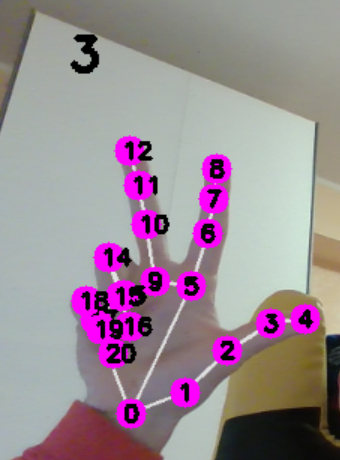
\includegraphics[height=0.4\linewidth]{immagini/mano.png}
    \hspace*{5pt}
    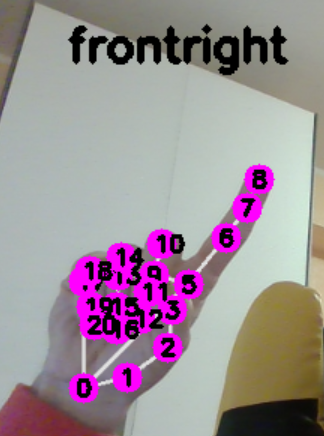
\includegraphics[height=0.4\linewidth]{immagini/mano_2.png}
    \caption{Esempi di gesture recognition}
\end{figure}

\subsubsection{Istruzioni sulle gesture}
Oltre ai due comandi principali che abbiamo appena spiegato, abbiamo implementato dei meccanismi di utilizzo basati su segni e azioni diverse che l'utente fa tramite la sua mano, ovvero:
\begin{itemize}
    \item \textbf{Cambio di modalità}: il cambio di modalità avviene portando l'indice al di sotto del polso.
    \begin{figure}[H]
        \centering
        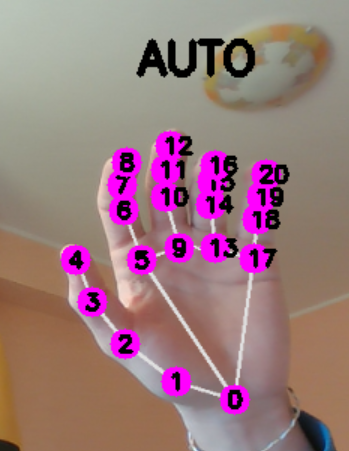
\includegraphics[height=0.4\linewidth]{immagini/mode_auto.png}
        \hspace*{5pt}
        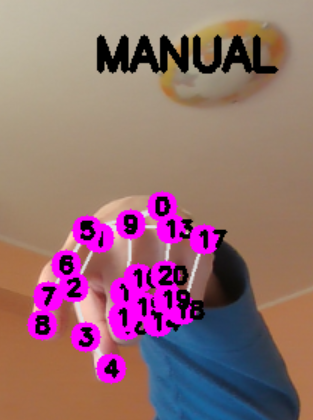
\includegraphics[height=0.4\linewidth]{immagini/cambio_mode.png}
        \caption{Esempio di cambio modalità}
    \end{figure}
    \item \textbf{Comando stop}: il comando stop viene impartito al robot chiudendo il pugno quando si è in modalità manuale. 
    \item \textbf{Cambio target}: in modalità automatica, invece, il pugno serve a cambiare posizione da raggiungere. Se l'utente ha indicato un numero, quindi chiude il pugno, allora il robot continuerà ad andare verso quel target. Non appena però l'utente apre nuovamente la mano, allora il robot si fermerà ed inizierà a calcolare il numero per la prossima direzione.
    \begin{figure}[H]
        \centering
        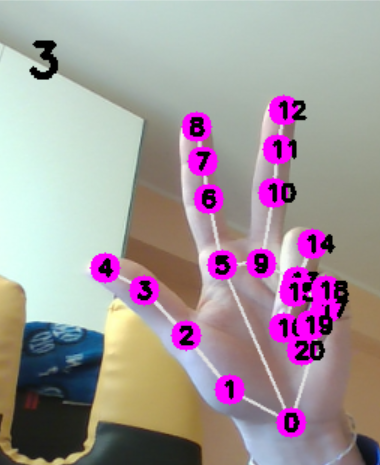
\includegraphics[height=0.37\linewidth]{immagini/esempio_mano_numero.png}
        \hspace*{5pt}
        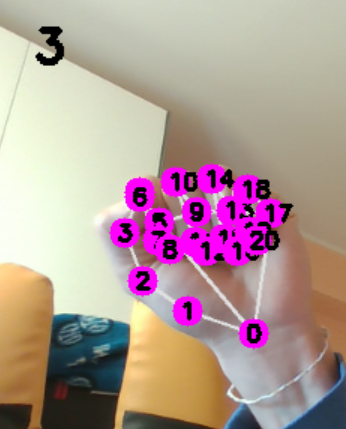
\includegraphics[height=0.37\linewidth]{immagini/esempio_mano_numero_pugno.png}
        \hspace*{5pt}
        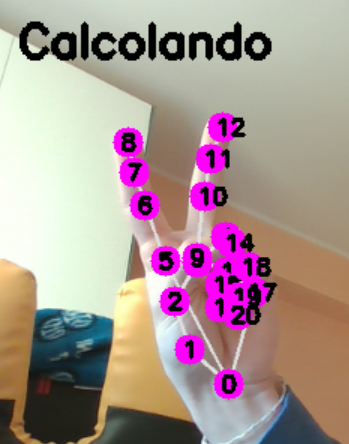
\includegraphics[height=0.37\linewidth]{immagini/esempio_mano_numero_calcolando.png}
        \caption{Esempio di cambio del target}
    \end{figure}
\end{itemize}



\subsection{Odometria}

Per via dell'incertezza del movimento dovuta alle varie caratteristiche fisiche del piano e del robot, abbiamo pensato ad un sistema che permette di calcolare la posizione del robot relativa all'arena tramite una griglia di tag ai quali è associata una certa coppia di coordinate.

\begin{figure}[H]
    \centering
    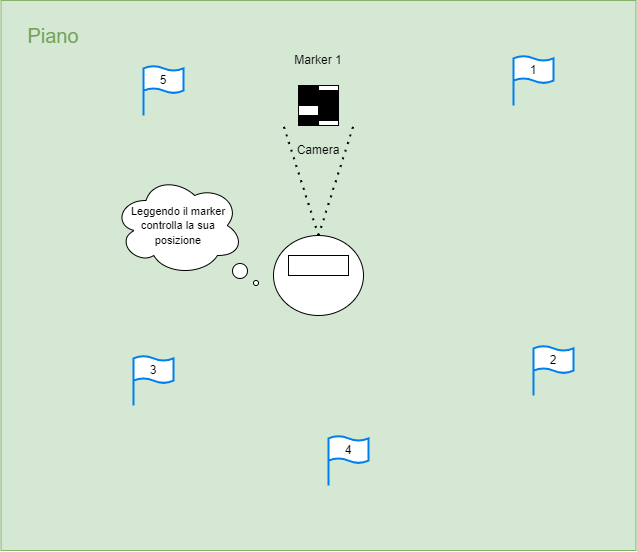
\includegraphics[width=0.6\linewidth]{immagini/diagramma_funzionamento_progetto.drawio.png}
    \caption{Rappresentazione del funzionamento del robot fisico}
\end{figure}

Ci siamo serviti del progetto \textbf{AprilTag} \cite{apriltags} dell'università del Michigan per i tag.
Questi tag sono stati sviluppati specificatamente per essere utilizzati nella robotica. Sono mosaici simili a dei QRcode, ma al contrario di quest'ultimi non contengo nessuna informazione.
Esistono diverse famiglie di tag e ognuna di esse associa ad ogni suo membro un id numerico univoco (noi abbiamo fatto uso della famiglia \textbf{36h11}).
I tag vengono acquisiti tramite la camera di bordo del robot e tramite l'omonima libreria C++\cite{apriltagscpp} possiamo poi calcolare una stima accurata della loro posizione nel piano.
    
\begin{figure}[H]
    \centering
    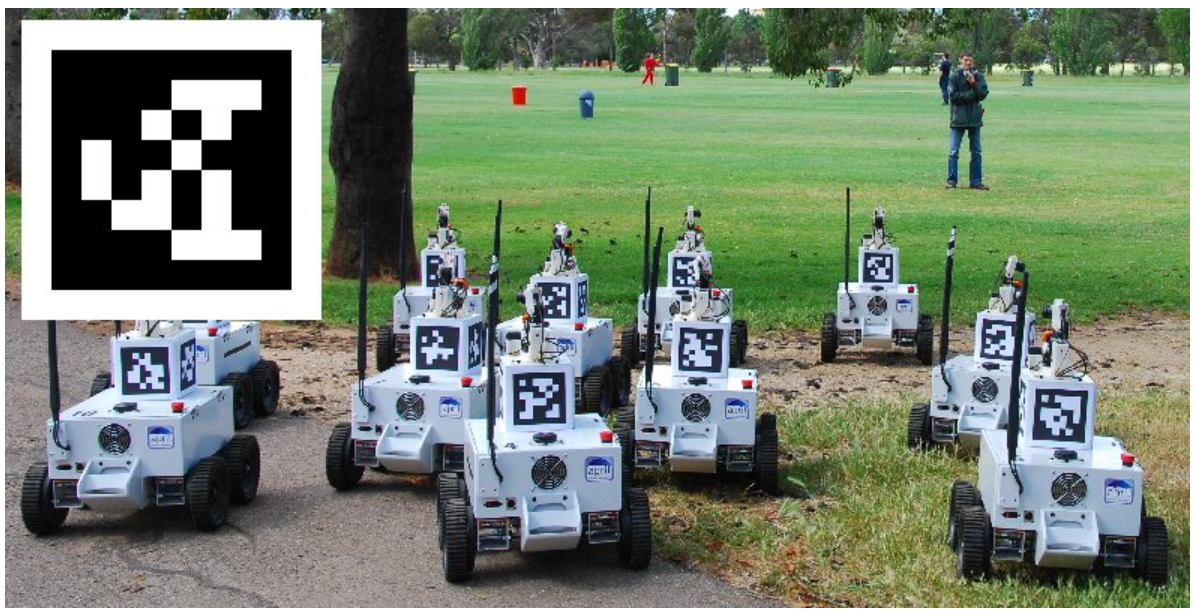
\includegraphics[width=0.5\linewidth]{immagini/AprilTag.png}
    \caption{Copertina AprilTags}
\end{figure}

\subsection{Obstacle avoidance}
Grazie a dei sensori di cui parleremo meglio in seguito, il robot è in grado di evitare gli ostacoli che gli si presentano di fronte. L'obiettivo principale è quindi quello di aggirare gli ostacoli mantenendo poi la direzione che si stava seguendo prima, intesa come posizione relativa rispetto al futuro orientamento del robot. Ad esempio, se il robot stava andando in direzione \texttt{FRONT} ma trova un ostacolo, dopo aver evitato l'ostacolo il robot continuerà ad andare nella direzione \texttt{FRONT}, che però non sarà la stessa direzione assoluta di prima a causa del nuovo orientamento del robot.


\pagebreak
\section{Tecnologie utilizzate}
\subsection{Software}
In questa sezione analizziamo le tecnologie utilizzate, i linguaggi e l'organizzazione del progetto.

\subsubsection{Organizzazione in moduli}
La nostra architettura è suddivisa in vari moduli, ciò rende l'intero sistema molto più flessibile.
La separazione netta del codice ci ha aiutati a ragionare più facilmente sulla logica di alto livello.
La gestione dei moduli avviene attraverso \textbf{Docker} \cite{docker}, questo software permette di creare ed organizzare
macchine virtuali chiamate container, tutti i moduli che non hanno bisogno di accedere direttamente all'hardware ed il broker MQTT operano all'interno di un loro container.
Questi approccio annulla completamente qalsiasi problema di compatibilità con la macchina host dato che ogni modulo ha effettivamente un suo sitema operativo.
Volendo grazie a Docker c'è anche la possibilità di distribuire i moduli su diversi elaboratori senza dover modificare in codice in alcun modo,
l'unico requisito è che gli elaboratori in questione siano in qualche modo collegati tra di loro, in una rete locale o via internet.


\subsubsection*{Moduli comuni tra le due versioni}
I moduli comuni (e pressoché invariati) tra la versione virtuale e quella fisica sono:
\begin{itemize}
    \item \textbf{Mosquitto}: container che utilizza l'immagine ufficiale di docker eclipse-mosquitto, permette a tutti gli altri moduli di comunicare.
    \item \textbf{Controller}: cervello del robot, elabora tutte le informazioni ricevute da gesture e sensori, quindi le trasforma in azioni per i motori del robot. Ci sono lievi differenze tra la versione fisica e quella virtuale dovute all'interfacciamento con l'ambiente di simulazione e al calcolo della posizione.
    \item \textbf{Perception}: modulo che si occupa di leggere i valori numerici dai sensori e trasformarli in \textit{free spaces} da restituire al controller.
\end{itemize}
In aggiunta abbiamo il modulo gesture, non contenuto all'interno di un container docker a causa dell'impossibilità su Windows di accedere alla webcam dall'interno di un container. Questo modulo ha il compito di rilevare i comandi dalla mano dell'utente, inviando l'operazione rilevata.

\subsubsection*{Moduli specifici per la versione virtuale}
In aggiunta ai servizi sopra citati, abbiamo anche:
\begin{itemize}
    \item \textbf{Sense}: legge i valori restituiti dai sensori di prossimità del simulatore e li pubblica sul broker.
    \item \textbf{Action}: legge dal broker i comandi inviati dal controller, quindi li applica al robot impostando la velocità delle due ruote.
\end{itemize}

\begin{figure}[H]
    \centering
    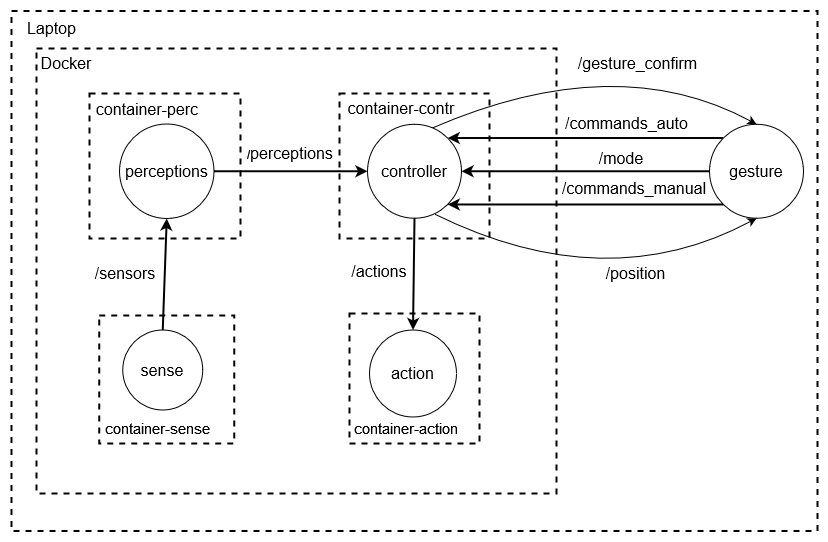
\includegraphics[width=0.7\linewidth]{immagini/comunicazione_moduli_virtuale.png}    
    \caption{Grafo delle comunicazioni tra i moduli nella versione virtuale}
\end{figure}

\subsubsection*{Moduli specifici per la versione fisica}
Nel caso fisico, invece, i moduli specifici sono eseguiti in processi separati sul Raspberry Pi dato che hanno bisogno di accedere all'hardware direttamente.
\begin{itemize}
    \item \textbf{Sense}: legge i valori restituiti su porta seriale dall'arduino, quindi li elabora e calcola i minimi per ogni settore (uno per ogni direzione di movimento del robot), infine li pubblica sul broker.
    \item \textbf{Action}: molto simile al modulo action della versione virtuale; legge l'ultimo comando pubblicato dal broker sul controller, quindi imposta la velocità lineare e la velocità angolare del robot.
    \item \textbf{Tag}: tramite la PiCamera, legge i valori del primo tag che rileva, successivamente esegue delle operazioni di image processing per migliorare il rilevamento e pubblica i dati calcolati sul broker, ovvero distanza e angolazione rispetto all'asse verticale.
\end{itemize}
Oltre a questi, un semplice script caricato sull'Arduino si occupa del funzionamento e della lettura dati dei sonar.

\begin{figure}[H]
    \centering
    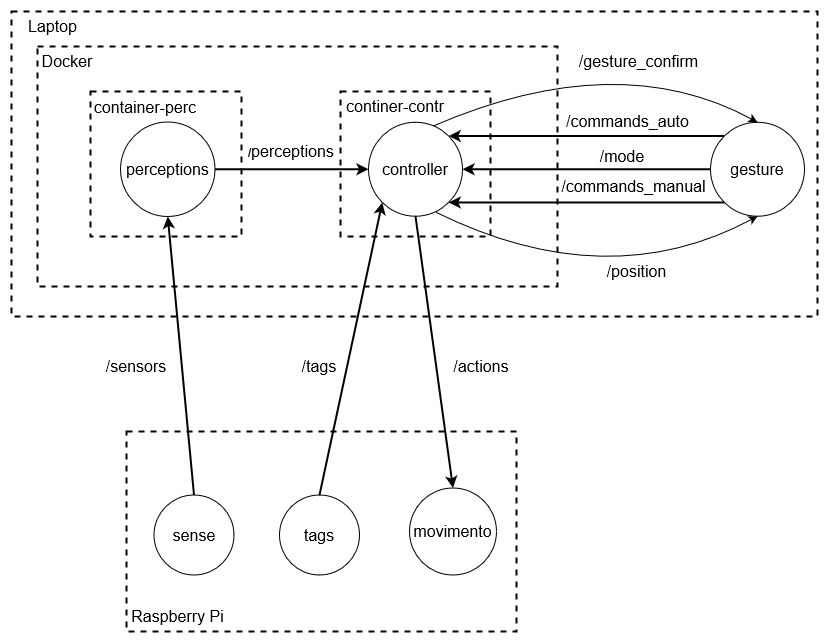
\includegraphics[width=0.7\linewidth]{immagini/comunicazione_moduli_fisico.png}
    \caption{Grafo delle comunicazioni tra i moduli nella versione virtuale}
       
\end{figure}

\subsubsection{Protocollo di comunicazione}
La comunicazione tra moduli avviene tramite MQTT. Ci siamo affidati a questo protocollo per la sua semplicità ed efficienza, inoltre si adatta perfettamente anche ad un progetto di piccola scala come il nostro.
Grazie ad MQTT è possibile inviare e ricevere dati su canali distinti, questo ci ha permesso separare logicamente il flusso delle informazioni rendendo il codice più robusto e sicuro.
Abbiamo preso in considerazione tutti i protocolli visti durante il corso: ROS/ROS2 ha diversi benefici però la grande complessità aggiunta ci ha portato ad escluderlo;
il PubSub con Redis svolge all'incirca lo stesso compito di MQTT e tra i due abbiamo preferito quello con cui avevamo più familiarità.
La scelta è ricaduta naturalmente sul protocollo MQTT.
Essendo estremamente diffuso (di fatto uno standard dell'industria), si può facilmente trovare l'implementazione di un client in un qualunque linguaggio di programmazione come ad esempio la libreria Paho
che utilizziamo sia in Python che in C++.

\subsubsection*{Messa in funzione del container mosquitto}
La creazione del container contenente il broker mosquitto è stata piuttosto lineare e può essere replicata seguendo i seguenti passaggi:
\begin{enumerate}
    \item Creazione del container all'interno del compose, inserendo nel file docker-compose.yml il seguente codice:
    \begin{figure}[H]
        \centering
        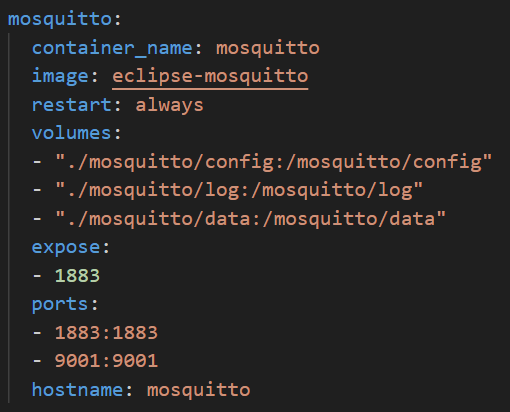
\includegraphics[width=0.3\linewidth]{immagini/mosquitto_nel_docker_compose.png}
    \end{figure}
    \item Creazione della cartella mosquitto con la seguente struttura all'interno della stessa cartella contenente il docker-compose.yml:
    \begin{figure}[H]
        \centering
        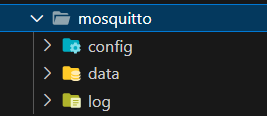
\includegraphics[width=0.2\linewidth]{immagini/struttura_cartelle_mosquitto.png}        
    \end{figure}
    \item Creazione di un file mosquitto.conf all'interno della cartella config contenente le seguenti impostazioni:
    \begin{center}
        \begin{verbatim}
            persistence true
            persistence_location /mosquitto/data/
            
            log_dest file /mosquitto/log/mosquitto.log
            log_dest stdout
            
            listener 1883
            
            password_file /mosquitto/config/mosquitto.passwd
            allow_anonymous false
        \end{verbatim}
    \end{center}
    \item \textbf{Creazione delle utenze (opzionale)}: esecuzione dei comandi 
    \begin{verbatim}
        docker compose up -d mosquitto & docker exec -it mosquitto sh
    \end{verbatim}
    per l'apertura di una shell all'interno del container, quindi creazione di un'utenza tramite il comando 
    \begin{verbatim}
        mosquitto\_passwd -c /mosquitto/config/mosquitto.passwd nome\_utente
    \end{verbatim}
    L'opzione -c serve solo quando si crea il primo utente per creare il file mosquitto.passwd. Se si sceglie di saltare questo passaggio, bisogna eliminare le ultime due righe nel file mosquitto.conf.

\end{enumerate}

\subsubsection{Linguaggi utilizzati}

I linguaggi utilizzati in questo progetto sono Python e C++. In particolare, la parte virtuale è scritta completamente in Python, mentre nella parte fisica i moduli Action, Sense e lo script sull'Arduino sono scritti in C++.

\begin{table}[htbp]
    \centering
    \begin{tabular}{|c|c|c|}
        \hline
        Modulo       & Virtuale & Fisico \\
        \hline
        Controller   & Python   & Python \\
        Gesture      & Python   & Python \\
        Perception   & Python   & Python \\
        Action       & Python   & C++    \\
        Sense        & Python   & Python \\
        Tags         & -        & C++    \\
        Script sonar & -        & C++    \\
        \hline
    \end{tabular}
    \caption{Linguaggi utilizzati nei moduli}

\end{table}

\subsubsection{Librerie e software di terze parti}

\begin{description}
    \item[Docker]: software di virtualizzazione molto popolare per la sua versatilità, permette di creare macchine virtuali minimali ed efficienti, ne facciamo uso per modularizzare il nostro sistema.
    \item[OpenCV]: famosa libreria open-source di computer vision, fondamentale sia nel rilevamento dei tag che nella gesture recognition.
    \item[AprilTags]: libreria C++ che serve a rilevare gli omonimi tag e a stimarne distanza ed angolazione.
    \item[Mediapipe]: suite di machine learning fornita da Google. Utilizziamo la libreria di gesture recognition in Python per dare comandi al robot.
    \item[OpenNI SDK]: software development kit di Orbbec che sfruttavamo per accedere alla videocamera Astra.
    \item[Kobuki SDK]: software development kit per Kobuki, ne facciamo uso per dare gli effettivi comandi di movimento alla base.
    \item[libcamera]: ambizioso progetto open-source creato dalla comunità Linux nel 2018 con lo scopo sostituire completamente gli attuali driver per le videocamere che necessariamente devono utilizzare codice closed-source. Noi la utilizziamo per interfacciarci con la PiCamera.
    \item[Paho MQTT]: client MQTT \cite{mosquitto} sviluppato da Eclipse, lo usiamo sia in Python che in C++ per far comunicare i moduli dell'architettura a microservizi.
    \item[CoppeliaSim]: simulatore di robot utilizzato anche a livello industriale, nonostante ciò non richiede harware particolarmente potente.
    \item[API CoppeliaSim]: client basato su ZeroMQ, ci ha permesso di interagire con la simulazione da remoto.
    \item[Arduino]: framework per programmare board dell'omonimo marchio, ne facciamo uso tramite l'estensione PlatformIO di VSCode per progrmmare l'Arduino Nano che controlla il sonar.
\end{description}


\subsubsection{Simulazione}
Per simulare il nostro robot abbiamo deciso di servirci di CoppeliaSim, un simulatore di robot con cui abbiamo familiarizzato durante il corso.
La parte virtuale del nostro progetto utilizza il robot Pioneer, questo robot a due ruote è stato scelto perché molto simile alla base kobuki usata nella parte fisica del progetto.
Dato che il movimento in un ambiente simulato non ha errori non è necessario alcun meccanismo di odometria. La posizione esatta del robot può essere ricavata in ogni momento grazie all'API di Coppelia. 
\begin{figure}[H]
    \centering
    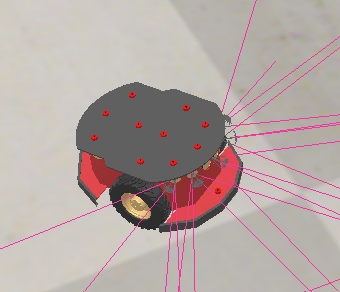
\includegraphics[width=0.4\linewidth]{immagini/PioneerRobot.png}
    \caption{Pioneer robot}
\end{figure}
Il robot utilizza cinque sensori di prossimità, con un cono ampio 36\textdegree\ per il sensore frontale e 43\textdegree\ per tutti gli altri. Infine, utilizza due motori, uno per ogni ruota. 


\subsection{Hardware}

Abbiamo scelto la base Kobuki come piattaforma principale del nostro progetto, una piattaforma mobile dotata di motori a trazione differenziale e diversi sensori integrati (che non trattiamo nel nostro progetto). Oltre alla base Kobuki, impieghiamo diversi sensori ed attuatori per implementare obstacle avoidance ed odometria.
I comandi movimento verranno impartiti tramite l'apposito SDK implementato in C++\cite{kobukisdk}.
\begin{figure}[H]
    \centering
    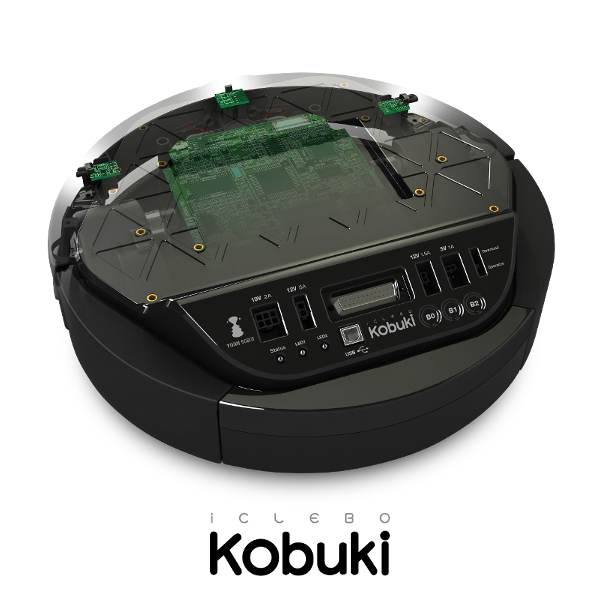
\includegraphics[width=0.3\linewidth]{immagini/kobuki.png}
    \caption{Robot Kobuki}
\end{figure}

\subsubsection{Sensori}
Per implementare tutte le funzionalità specificate, il robot richiede:
\begin{itemize}
    \item \textbf{Fotocamera} Astra di Orbbec/PiCamera per la lettura dei tag.
    \item \textbf{Sensori di prossimità} a ultrasuoni HC-SR04.
    \begin{figure}[H]
        \centering
        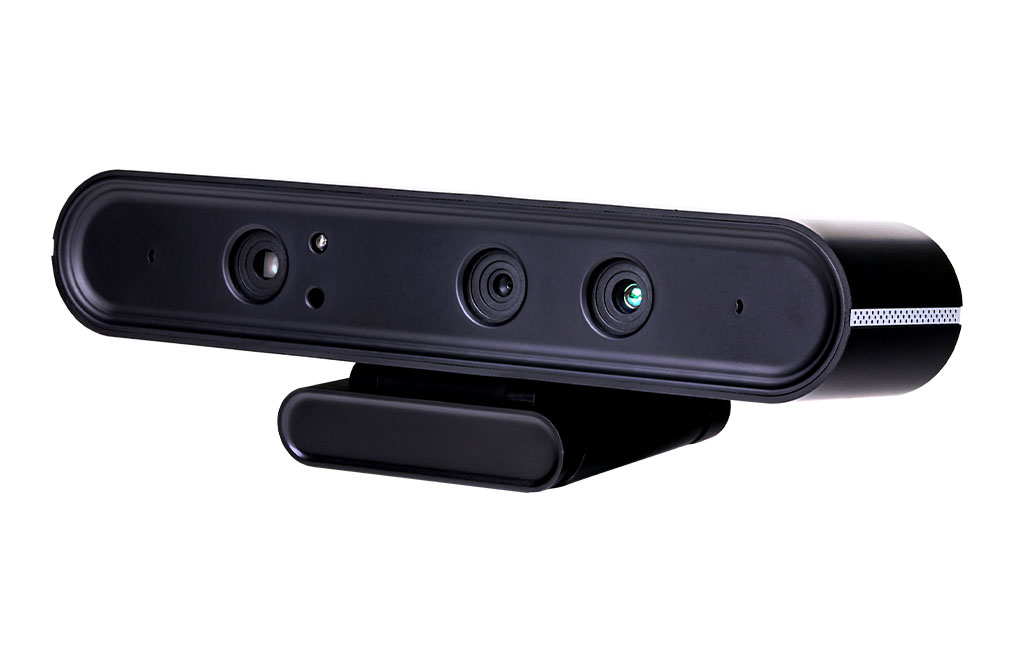
\includegraphics[height=0.18\linewidth]{immagini/astra_orbbec_s.jpg}
        \hspace*{5pt}
        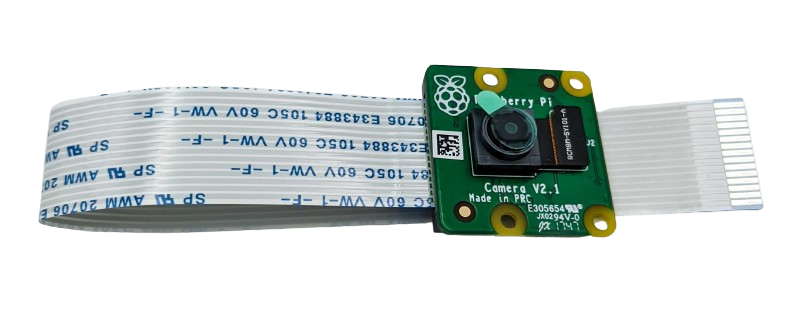
\includegraphics[height=0.18\linewidth]{immagini/rpi-camera.png}
        \hspace*{5pt}
        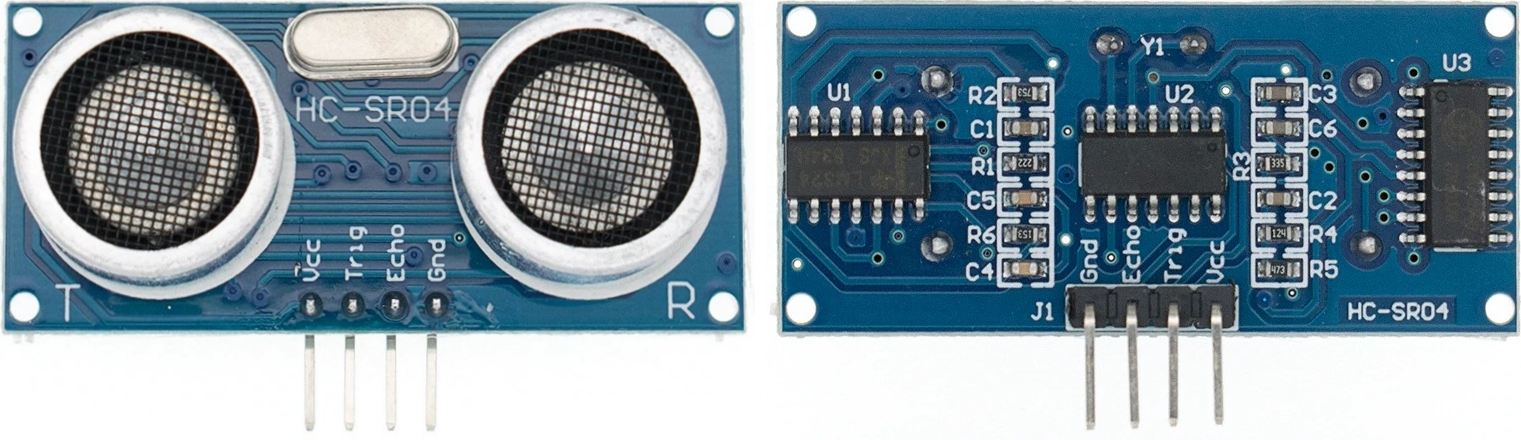
\includegraphics[height=0.1\linewidth]{immagini/HC-SR04.jpg}
        \caption{Sensori utilizzati}
    \end{figure}      
\end{itemize}


\subsubsection{Attuatori}

Sono necessari:
\begin{itemize}
    \item \textbf{Motori} per le due ruote (inclusi nella base Kobuki).
    \item \textbf{Servomotori} per i sonar.
        \begin{figure}[H]
            \centering
            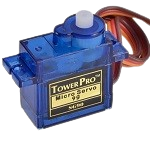
\includegraphics[height=0.2\linewidth]{immagini/servomotore.png}
            \hspace*{5pt}
            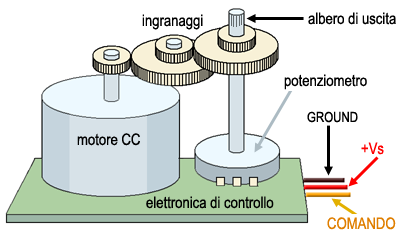
\includegraphics[height=0.2\linewidth]{immagini/servomotori_spiegazione.png}
            \caption{Attuatori}
        \end{figure}
\end{itemize}

\subsubsection{Unità di calcolo}
I dispositivi utilizzati per il calcolo e l'esecuzione del codice sono:
\begin{itemize}
    \item \textbf{Computer personale} utilizzato per il rilevamento delle gesture e per l'hosting dei moduli controller e perception. Nel caso del robot virtuale, l'intero progetto viene eseguito sul computer.
    \item \textbf{Raspberry Pi 3B+} utilizzato per i calcoli on-board del robot, come l'elaborazione delle immagini relative ai tag, dei dati dei sonar e l'invio dei comandi per il movimento.
    \item \textbf{Arduino nano} utilizzato per la messa in funzione dei sonar e per la lettura dei segnali elettrici dai servomotori e dai sensori HC-SR04.
        \begin{figure}[H]
            \centering
            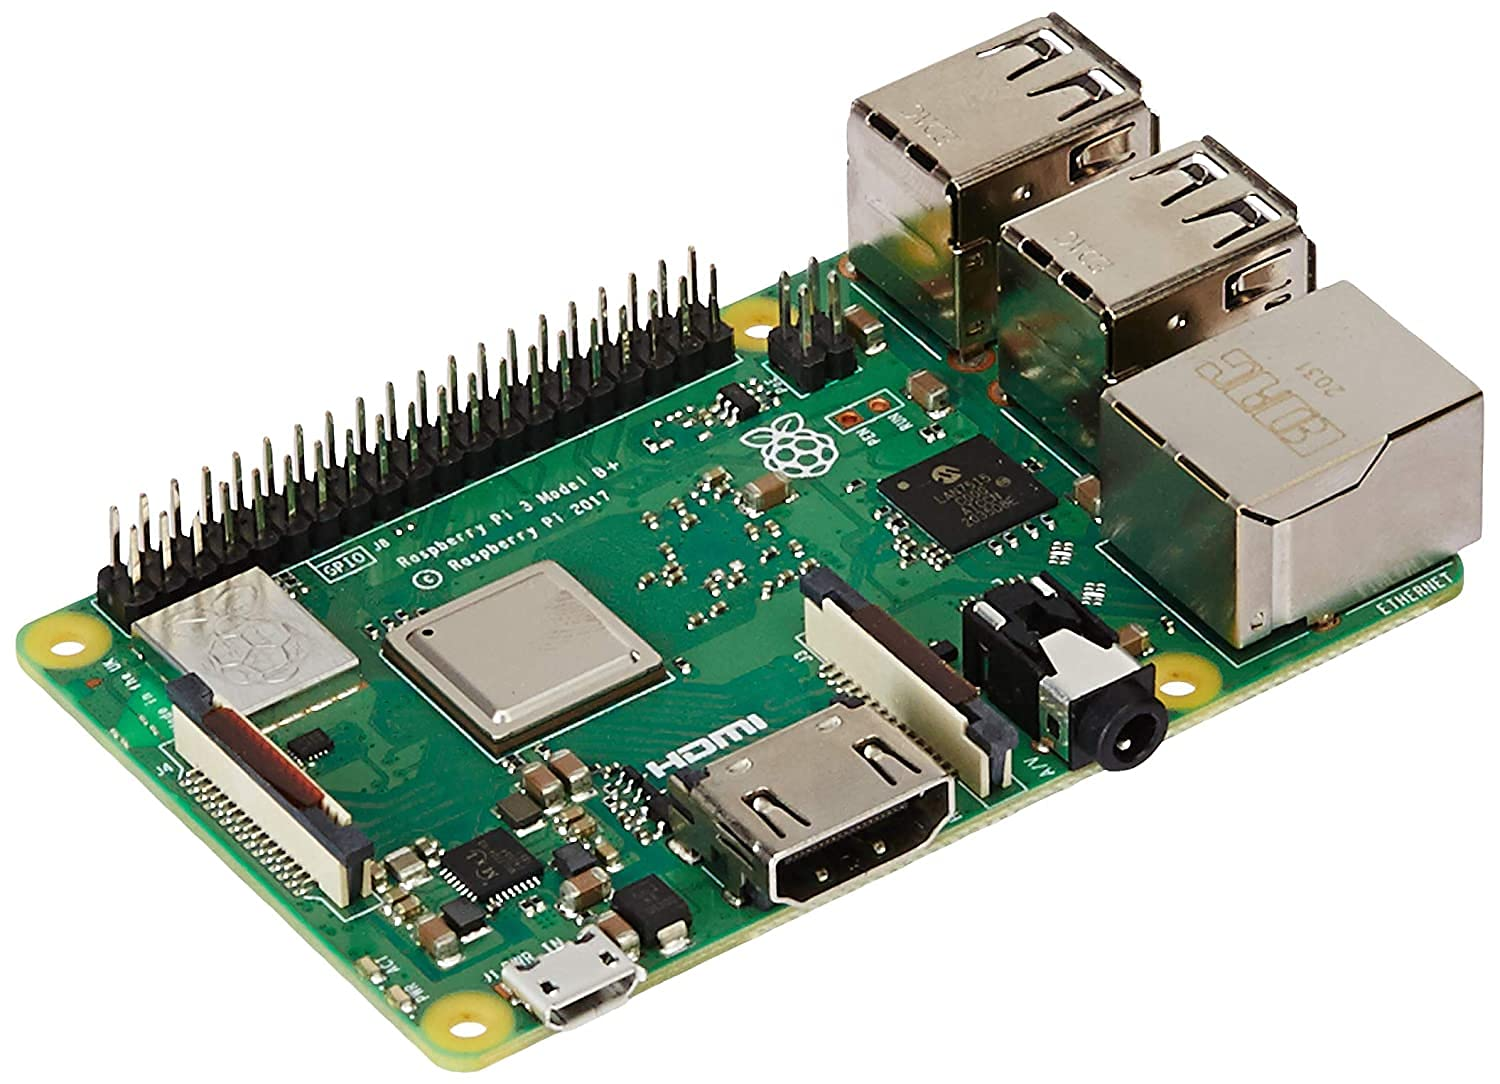
\includegraphics[width=0.3\linewidth]{immagini/rasapberry.jpg}
            \hspace*{5pt}
            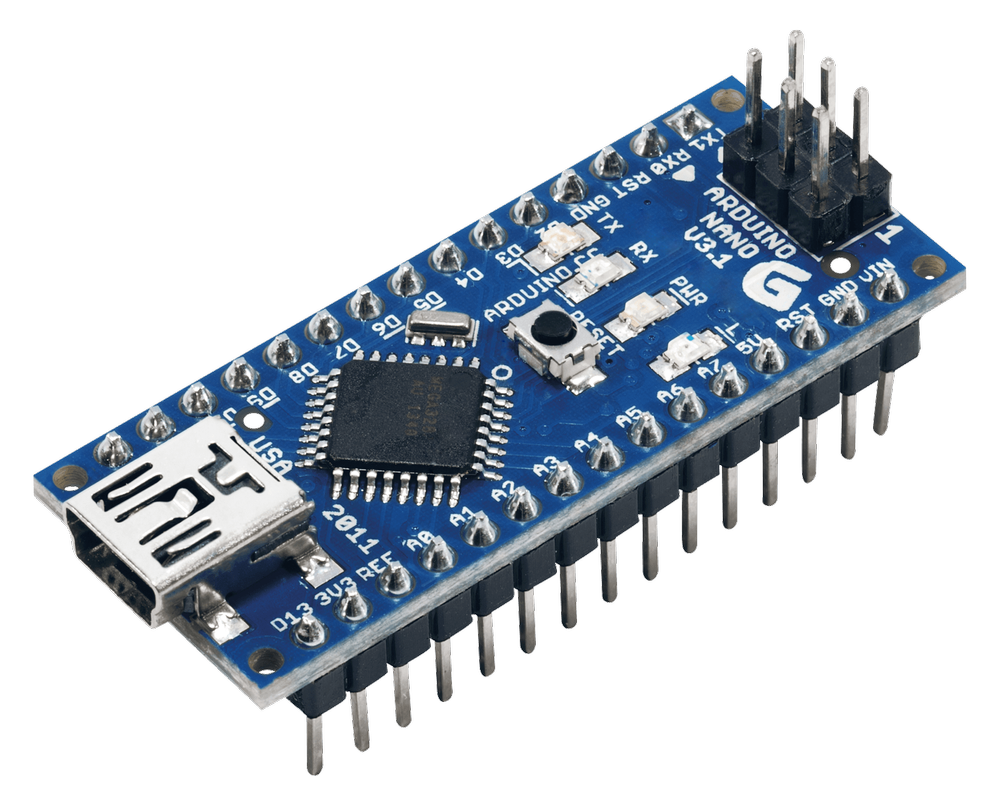
\includegraphics[width=0.2\linewidth]{immagini/arduino_nanp.png}
            \caption{Unità di calcolo utilizzate}
        \end{figure}

\end{itemize}



\pagebreak
\section{Punti critici}
In questa sezione analizziamo lo sviluppo di alcune criticità del nostro progetto, e tutte le scelte, gli errori e i problemi che ci hanno portato alla soluzione definitiva.

\subsection{Gesture recognition}
Il riconoscimento delle gesture è basato sull'estrazione da parte della libreria di 21 landmarks posizionati sulla mano, con relative coordinate. È stato quindi relativamente semplice creare meccanismi in grado di riconoscere gesture fatte dall'utente, come ad esempio la chiusura del pugno, la direzione verso cui indica la mano oppure il numero di dita aperte.

\subsubsection{Guida manuale}
La guida manuale si basa sull'imprimere una direzione al robot, oppure fermarlo. La direzione è stata calcolata prendendo come punti di riferimento i landmarks 0 (polso) e 8 (punta dell'indice), basandosi su due elementi:
\begin{itemize}
    \item Coefficiente angolare della retta passante per i due landmarks.
    \item Relazioni tra le coordinate dei due landmarks.
\end{itemize}
Assumiamo che quando l'ordinata dell'indice è minore dell'ordinata del polso, allora il comando non è supportato. Quando invece l'ordinata dell'indice è maggiore, allora ci sono diversi casi, a seconda dei valori del coefficiente angolare, ovvero:
\begin{itemize}
    \item \textbf{Se $\mathbf{m < 1}$}, allora la direzione è \textbf{left}.
    \item \textbf{Se $\mathbf{1 < m < 3}$}, allora la direzione è \textbf{frontleft}.
    \item \textbf{Se $\mathbf{m > 3}$ oppure $\mathbf{m < -3}$}, allora la direzione è \textbf{front}.
    \item \textbf{Se $\mathbf{-3 < m < -1}$}, allora la direzione è \textbf{frontright}.
    \item \textbf{Se $\mathbf{m > -1}$}, allora la direzione è \textbf{right}.
\end{itemize}

\begin{figure}[H]
    \centering
    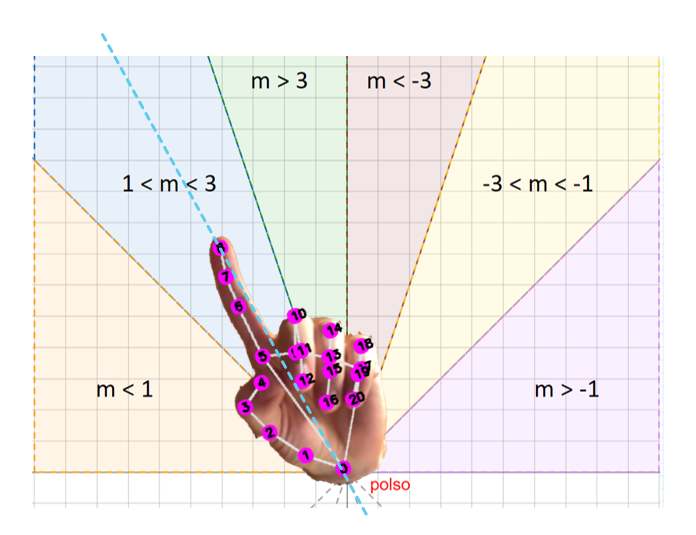
\includegraphics[height=0.5\linewidth]{immagini/calcolo_con_coeff_angolare_con_mano.png}
    \caption{Calcolo della direzione tramite coefficiente angolare}
\end{figure}

\subsubsection{Guida automatica}
Nella guida automatica, l'obiettivo è quello di calcolare il numero di dita aperte per poi restituire la posizione da raggiungere al controller. Anche nel caso del controllo che un dito sia aperto o meno, il calcolo viene fatto sulle posizioni dei vari landmarks. Prendiamo come esempio il dito indice:

\begin{figure}[H]
    \centering
    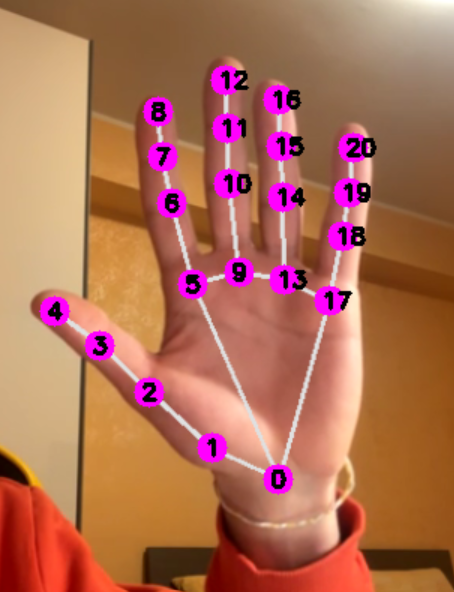
\includegraphics[height=0.6\linewidth]{immagini/mano_aperta.png}
    \caption{Disposizione dei landmarks sulla mano}
\end{figure}

Il controllo sull'apertura viene fatta basandosi sui landmarks 0, 6 e 8. In particolare, se la distanza tra 0 e 8 è maggiore di quella tra 0 e 6, allora il dito viene rilevato come aperto. Applicando questo ragionamento separatamente ad ogni dito, possiamo calcolare il numero delle dita aperte. Un ragionamento leggermente diverso va fatto sul pollice, poiché in questo caso la punta del pollice potrebbe non chiudersi sulla nocca dello stesso, ma verso l'alto. Per questo motivo, viene utilizzata come punto di riferimento la distanza con il landmark 17: se la distanza tra 4 e 0 è maggiore di quella tra 0 e 17, allora il pollice è aperto. Infine, questo conteggio viene utilizzato anche per rilevare la chiusura del pugno, utile anche nella guida manuale per fermare il robot.


\subsubsection*{Miglioramenti al calcolo del numero}
Dato che l'apertura della mano è un operazione potenzialmente lenta, abbiamo deciso di rendere il calcolo più consistente allungandone la durata. In particolare, viene calcolata una media pesata su 40 frame consecutivi, dove il peso è dato proprio dall'indice del frame. In questo modo, si va a dare maggiore importanza al numero calcolato sulla mano dopo un certo lasso di tempo.


\subsubsection{Cambio di modalità}
Il cambio di modalità avveniva inizialmente tramite l'utilizzo della seconda mano. Facendo il pugno con essa, la modalità veniva cambiata e si poteva quindi procedere ad impartire i comandi al robot con la mano principale. Tale soluzione risultava scomoda e poco efficace, quindi abbiamo optato per una soluzione senza l'utilizzo della mano secondaria. La soluzione finale è quella spiegata nell'introduzione, ovvero il posizionamento dell'indice al di sotto del landmark del polso.
Questo modo ci è sembrato più intuitivo.

\subsection{Movimento della base Kobuki}
La messa in movimento della base Kobuki viene fatta attraverso l'omonimo sdk in C++.

\subsubsection{Introduzione all'SDK}
Il robot Kobuki comunica con il Raspberry Pi tramite uno specifico protocollo USB, fortunatamente l'SDK in C++ fornito nella documentazione astrae completamente tale protocollo,
basta semplicemente collegarsi al dispositivo ed impostare le velocità desiderate per farlo muovere.

\subsubsection{Problemi con l'installazione}
L'installazione delle librerie richieste è avvenuta senza grossi problemi grazie all'ottima documentazione che spiega ogni singolo passo nel dettaglio.
L'unico problema riscontrato durante l'installazione è stato un errore di compilazione dovuto all'utilizzo dei \textbf{Variable Length Array}  (abbreviato VLA) nel codice
sorgente di alcuni moduli dell'SDK. Questa feature di C++ è ormai considerata obsoleta e pericolosa perciò non sembra andare d'accordo con le versioni più recenti del compilatore gcc
(noi usiamo la versione 12). Il tentativo di disattivare gli errori causati passando una serie flag al compilatore non è andato a buon fine. Infine ne siamo venuti a capo sostituendo i VLA con
std::vector nei file indicati degli errori, questo ha definitivamente risolto il problema, il resto dell'installazione è proseguita a gonfie vele. 

\subsubsection{Odometria integrata}
La base Kobuki fornisce diverse funzioni, tra cui un sistema di odometria integrata che abbiamo tentato di integrare nel nostro progetto. Inizialmente avevamo pensato di usarlo come una sorta di backup al sistema basato su AprilTag.
Purtroppo questa funzione sembra essere molto instabile, si attiva solo dopo un certo lasso di tempo e restituisce valori con un grosso margine di errore.
Non avendo il tempo di approfondire abbiamo completamente abbandonato l'idea.


\subsection{Odometria}
Fin da subito abbiamo scelto di affidarci agli AprilTags per il calcolo della posizione. Per il rilevamento di suddetti tag abbiamo inizialmente utilizzato la camera Astra Series di ORBBEC.
Il concetto si basa sulla disposizione dei tag sul pavimento in modo da formare una griglia $4 \times 4$. Ad ogni tag viene associato un indice ed una coppia di coordinate, tramite la forma polare delle coordinate, il robot riesce a calcolare la propria posizione.
La stima della posizione tramite tag ha una precisione paragonabile ad altri metodi di odometria che abbiamo considerato e poi scartato, in più non richiede dispositivi particolari, basta una semplice videocamera che non abbia troppo motion blur.

\subsubsection{Messa in funzione della videocamera}

La videocamera Astra non sembra essere compatibile con Video4Linux2, il driver incluso nel sistema operativo che si occupa proprio di interagire con le periferiche di cattura delle immagini.
Il dispositivo veniva rilevato correttamente come videocamera quando collegata via USB ma era impossibile comunicare con essa tramite Linux.
Tutto ciò ha ci ha impedito di utilizzare qualsiasi tipo di libreria che si interfacciasse con le videocamere tramite V4L2, come ad esempio OpenCV.
Siamo quindi dovuti ricorrere allo standard OpenNI2 \cite{opencvopenni} specifico per videocamere con sensore di profondità come Astra.
Come primo passo abbiamo tentato di integrare OpenNI2 con OpenCV \cite{opencvastra} ricompilando la libreria seguendo l'apposita documentazione. Quest'approccio non ha dato risultati
, OpenNI2 viene utilizzato da OpenCV solo per il sensore di profondità, mentre per il sensore ottico a colori si appoggia comunque a V4L2.
Successivamente siamo ricorsi all'SDK (sempre basato su OpenNI) \cite{orbeccsdk} messo a disposizione da Orbbec per comunicare direttamente tramite USB, scavalcando quindi il sistema operativo.
Nonostante una documentazione praticamente inesistente siamo riusciti ad installare l'SDK e tramite alcuni esempi abbiamo finalmente estratto dei fotogrammi a colori dalla camera.

\subsubsection{Calcolo della posizione dai dati del tag}
Le informazioni che ricaviamo dal tag inquadrato sono:
\begin{itemize}
    \item \textbf{Distanza} tra la videocamera e l'angolo in alto a sinistra del tag.
    \item \textbf{Angolo (yaw)} tra il versore (0,-1) e il vettore che va dal vertice in basso a sinistra (bottom\_sx) e il vertice in alto a sinistra (top\_sx).
          \begin{figure}[H]
              \centering
              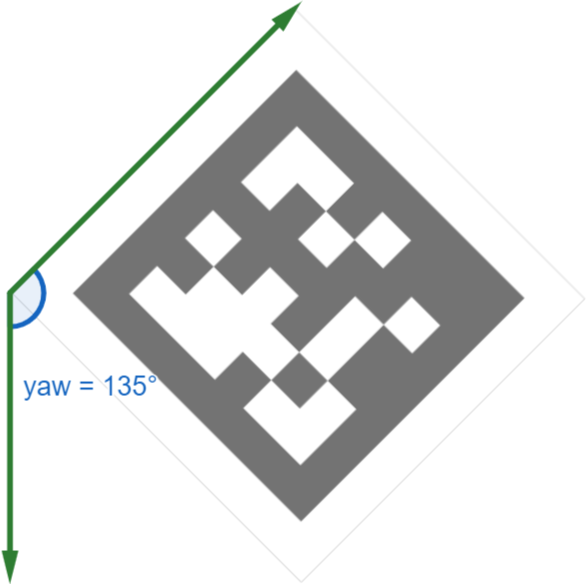
\includegraphics[height=0.3\linewidth]{immagini/yaw.png}
              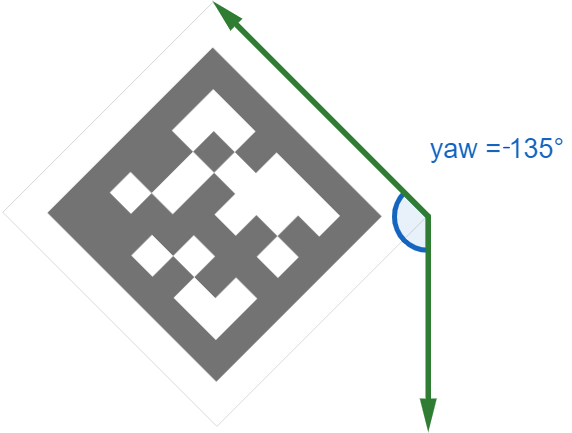
\includegraphics[height=0.3\linewidth]{immagini/spiegazione_yaw_negativo.png}
              \caption{Spiegazione angolo yaw}
          \end{figure}
          Questo angolo va da -180 a 180 ed ha segno positivo se la punta del vettore si trova più a destra rispetto alla base, altrimenti segno negativo.
    \item \textbf{Angolo (phi)} tra il centro della videocamera e il punto in cui si trova il tag.
          \begin{figure}[H]
              \centering
              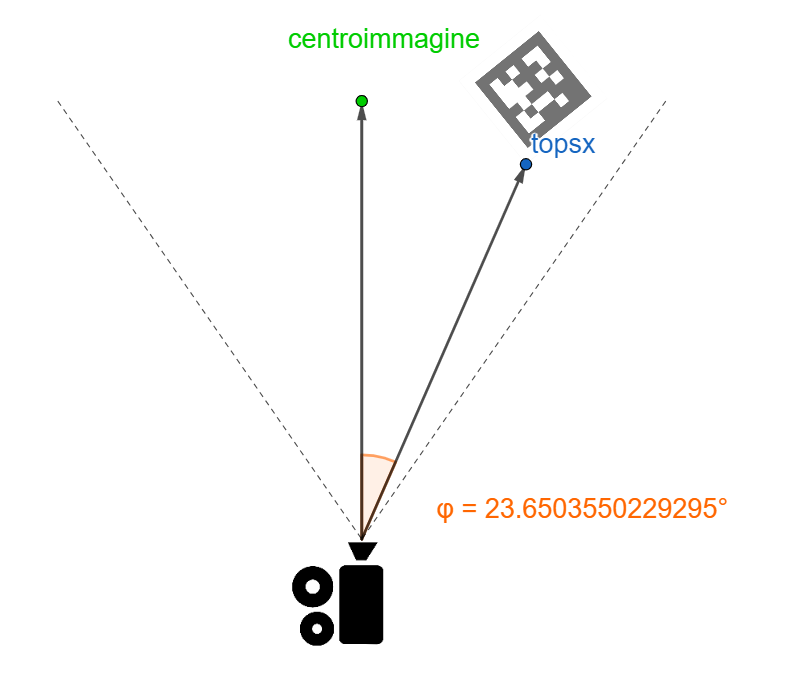
\includegraphics[height=0.3\linewidth]{immagini/phi_positivo.png}
              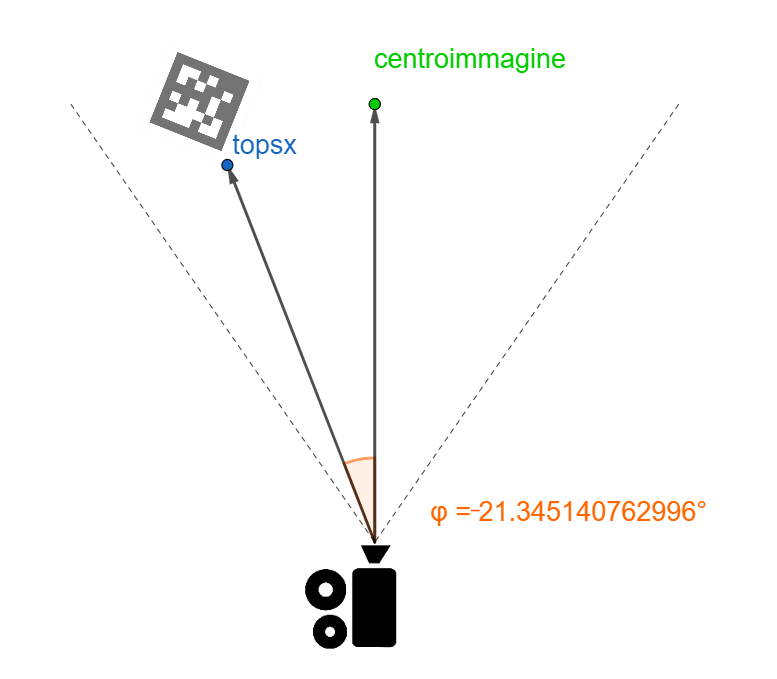
\includegraphics[height=0.3\linewidth]{immagini/phi_negativo.png}
              \caption{Spiegazione angolo phi}
          \end{figure}
\end{itemize}

Il calcolo dell'orientamento del robot rispetto all'angolo 0 (verso destra) viene sempre fatto tenendo conto di phi e yaw. Le casistiche possono essere diverse; ad esempio, nel caso in cui il robot si trovi come in figura
\begin{figure}[H]
    \centering
    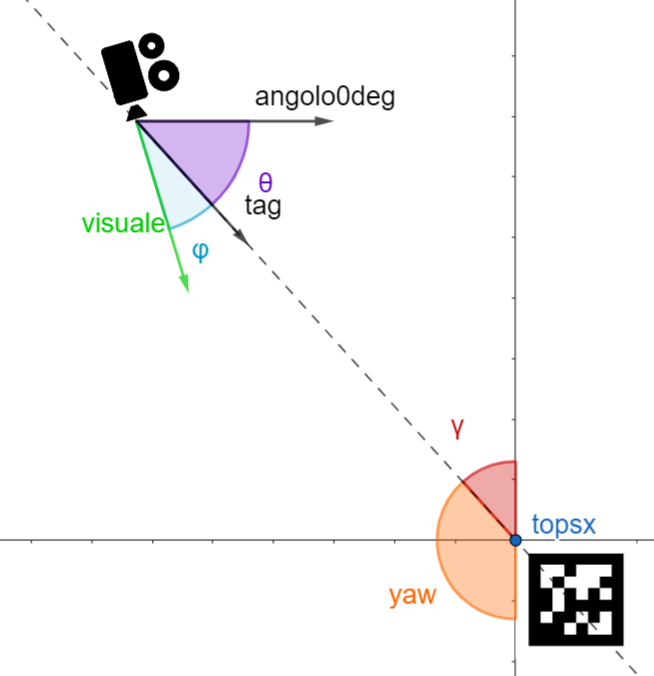
\includegraphics[height=0.4\linewidth]{immagini/calcolo_orientamento.png}
    \caption{Calcolo orientamento rispetto all'angolo 0}
\end{figure}
allora l'orientamento può essere calcolato come $-(\phi + \theta)$. Successivamente, si passa a calcolare la posizione della camera tramite applicazioni di geometria e trigonometria.
\begin{figure}[H]
    \centering
    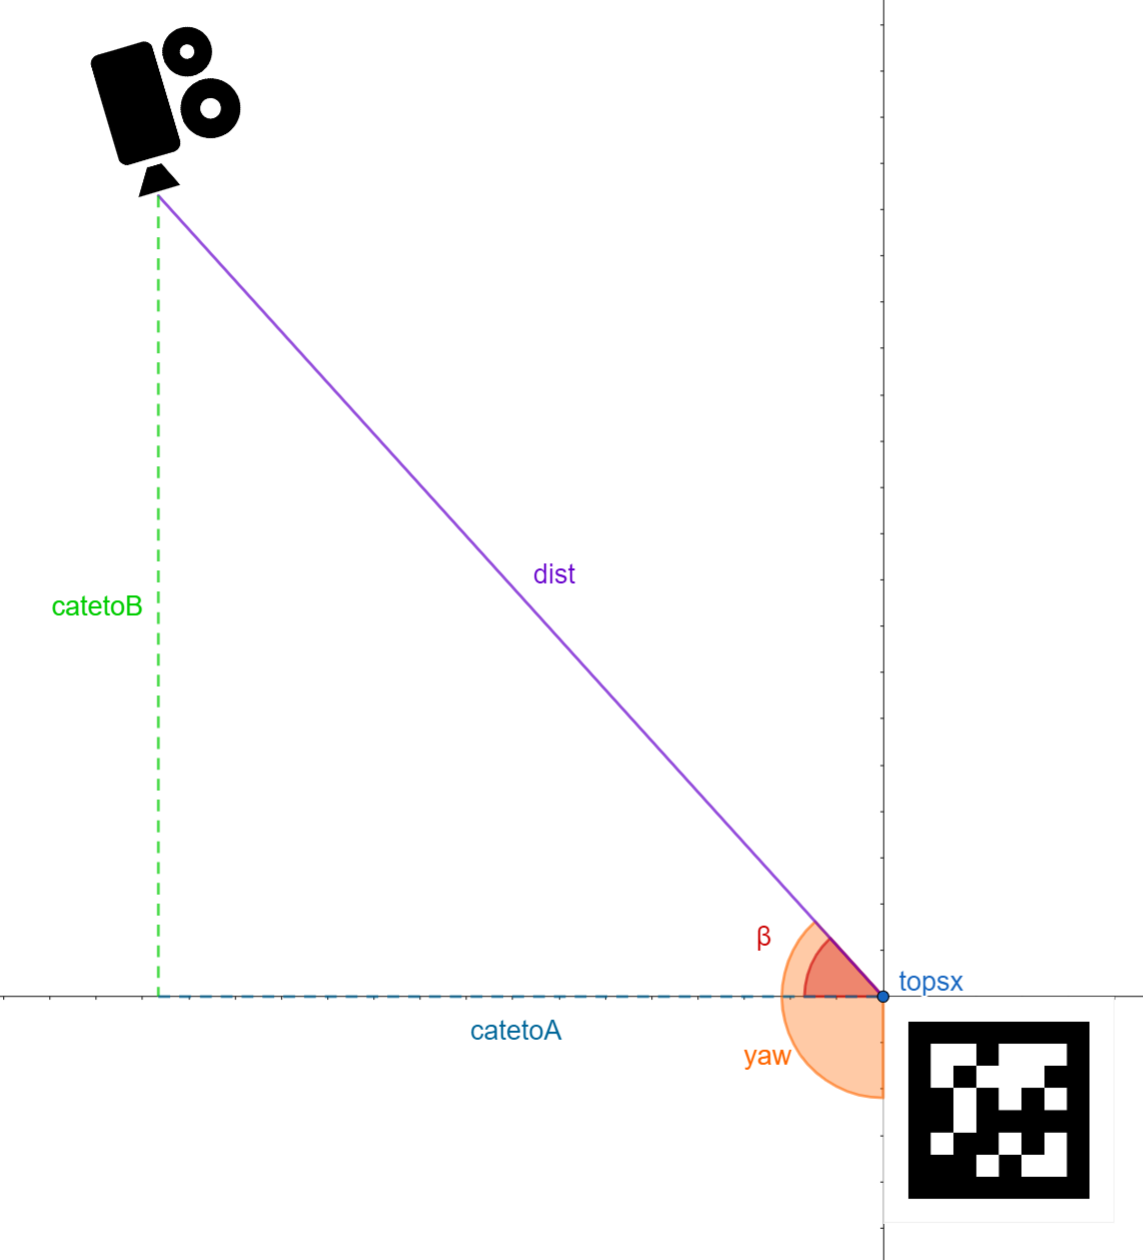
\includegraphics[height=0.5\linewidth]{immagini/calcolo_posizione.png}
    \caption{Calcolo posizione della camera}
\end{figure}
In questo esempio, possiamo facilmente calcolare le coordinate della camera partendo da yaw, distanza e coordinate del marker $(x\_m, y\_m)$ nel seguente modo:
\begin{equation}
    \beta = |yaw|\ \% \ 90
\end{equation}
\begin{equation}
    catetoA = dist\cdot cos(\beta)
\end{equation}
\begin{equation}
    catetoB = \sqrt{dist ^ 2 - a ^ 2}
\end{equation}
\begin{equation}
    x\_camera = x\_m - catetoA,\ \ \ y\_camera = y\_m + a
\end{equation}
Infine, conoscendo la posizione della camera, il raggio del robot e l'angolo phi si può facilmente, tramite calcoli simili, ottenere la posizione del centro del robot.

\subsubsection{Tag non paralleli alla camera}
Una volta che la camera è stata messa in funzione, siamo riusciti a leggere i tag direttamente durante il movimento. La libreria di AprilTags permette di eseguire diverse operazioni, in primis la detection dei tag. Per favorire tale operazione, abbiamo eseguito delle modifiche all'immagine in modo da renderla più pulita e nitida, ovvero:

\begin{enumerate}
    \item Conversione dell'immagine in scala di grigi.
    \item Sharpening per migliorare i bordi del tag tramite convoluzione con il kernel $$\begin{bmatrix}
                  -0.5 & -0.5 & -0.5 \\
                  -0.5 & 5    & -0.5 \\
                  -0.5 & -0.5 & -0.5 \\
              \end{bmatrix}$$
    \item Thresholding con una soglia pari a un'intensità di grigio media (110 circa).
\end{enumerate}
In questo modo, la detection aveva un tasso di fallimento notevolmente minore, il quale prima era più basso a causa della scarsa risoluzione della camera. La seconda operazione da noi utilizzata della libreria AprilTags è quella di ricavare facilmente dal tag rilevato la distanza e la rotazione sui tre assi (yaw, pitch e roll). Ci siamo concentrati sul primo di questi, ovvero sulla rotazione sull'asse verticale, pensando 
coincidesse con la variazione di orientamento tra la camera e il tag rispetto al piano. In realtà ci siamo resi conto ben presto che, a causa dell'inclinazione della camera (circa 40°), l'immagine del tag appariva distorta, portando quindi ad un errore significativo nello yaw. Abbiamo risolto questo problema applicando una serie di trasformazioni sull'immagine nel seguente ordine:
\begin{enumerate}
    \item Individuazione e ritaglio del rettangolo in cui è inscritto il tag.
    \item Interpolazione su tale rettangolo per renderlo quadrato.
    \item Sharpening sull'immagine interpolata per rimuovere l'effetto a "dente di sega" dai bordi.
    \item Operazione di apertura morfologica.
\end{enumerate}
Tramite queste operazioni andiamo a simulare che la camera si trovi in parallelo rispetto al pavimento e, quindi, rispetto al tag. Di conseguenza, l'orientamento rispetto all'asse verticale è esattamente l'orientamento rispetto al piano che cercavamo, con un margine di errore insignificante ai fini del nostro obiettivo.


\begin{figure}[H]
    \centering
    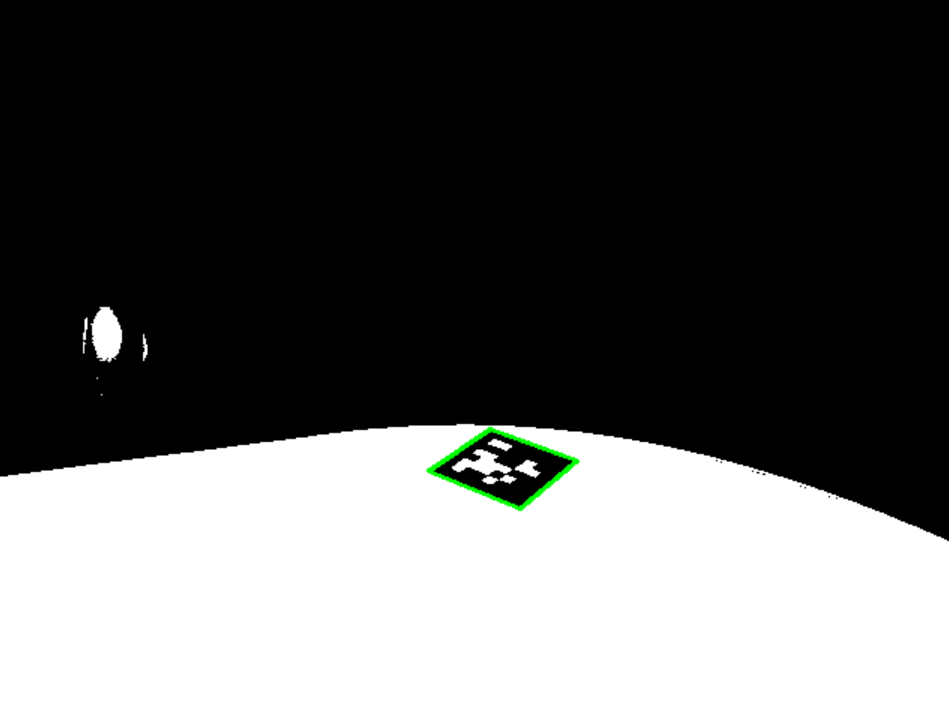
\includegraphics[height=0.3\linewidth]{immagini/stretching_tag_immagine_binarizzata.png}
    \hspace*{15pt}
    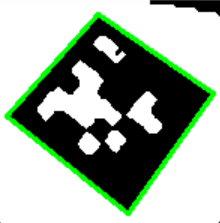
\includegraphics[height=0.3\linewidth]{immagini/tag_stretchato.png}
    \caption{Detection degli AprilTags}
\end{figure}

In questo caso si può vedere a sinistra l'immagine originale, alla quale è stato applicato un thresholding per migliorare il rilevamento andando ad aumentare il contrasto e a destra il tag interpolato che simula la posizione della camera parallela ad esso.

\subsubsection{Sostituzione della camera}
A pochi giorni dalla consegna del progetto, la camera Astra di Orbbec che stavamo utilizzando ha \textbf{inspiegabilmente} smesso di funzionare. Ciò ci ha obbligati a trovare una soluzione alternativa in poco tempo che avesse la stessa qualità della Astra. Dopo svariati tentativi, abbiamo optato per una PiCamera \cite{picam}.
In maniera simile ad Astra anche la PiCamera nonostante venga riconosciuta da V4L2 non è utilizzabile tramite OpenCV, questo probabilmente è dovuto al fatto che la libreria
che serve a dialogare con il dispositivo è stata deprecata del tutto \cite{newdriver} (nelle versioni più recenti di raspbian come la nostra è stata rimossa completamente) e sostituita con \textbf{libcamera} \cite{libcamera},
un libreria più moderna e senza dipendenza da codice proprietario. Visto il poco tempo rimanente e l'esperienza accumulata con la vecchia videocamera abbiamo deciso di proseguire direttamente con libcamera.
Una volta capito come includere ed utilizzare la nuova libreria abbiamo sostituito il codice e abbiamo iniziato ad ottimizzare la cattura dei tag.

\subsubsection{Rimozione della seconda detection}
Nonostante le operazioni mirate al miglioramento dell'immagine ritagliata sul tag a seguito dell'interpolazione, abbiamo notato che spesso la detection falliva proprio causa della qualità ancora troppo bassa di tale immagine. Questo motivo, insieme a questioni legate al tempo di esecuzione, ci ha spinti nel cambiare approccio per la risoluzione del problema del tag non parallelo alla camera.
Abbiamo pensato che, essendo noi in possesso delle informazioni sui quattro vertici del tag all'interno dell'immagine, potessimo eseguire un calcolo algebrico su tali valori, invece di richiedere una seconda detection alla libreria AprilTags. Questo ci avrebbe portato due vantaggi:
\begin{itemize}
    \item Riduzione del tasso di fallimento dovuto alla scarsa qualità dell'immagine ritagliata e interpolata.
    \item Azzeramento del tempo di esecuzione di ritaglio, interpolazione, sharpening e detection, seppur già minimo grazie alle ridotte dimensioni dell'immagine ritagliata.
\end{itemize}

\subsubsection*{Calcoli eseguiti}
Lo scopo del ragionamento che abbiamo fatto era quello di eseguire una sorta di interpolazione sui vertici, quindi calcolare manualmente l'orientamento del tag utilizzando i vertici nelle nuove posizioni, senza ricorrere alla libreria. Per fare ciò abbiamo eseguito i seguenti passaggi:
\begin{enumerate}
    \item La libreria restituisce le coordinate dei vertici all'interno di un array ordinato sempre nel seguente modo:
    \begin{figure}[H]
        \centering
        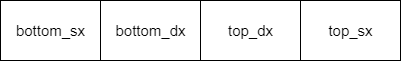
\includegraphics[width=0.5\linewidth]{immagini/array_vertici.png}
        \caption{Array dei vertici del tag}
    \end{figure}
    
    \item Sottraiamo a tutti e quattro i punti il valore min\_x alle ascisse e min\_y alle ordinate, in modo da poter trattare le coordinate dei vertici relativamente al box, ovvero al rettangolo in cui è inscritto il tag nell'immagine.
    \item Per eseguire l'interpolazione sui vertici, ci serve di sapere su che lato del box si trova ogni vertice. Per mantenere tale informazione, utilizziamo una variabile contenente l'indice del punto con ascissa 0 (come già detto, relativamente al box).
        \begin{figure}[H]
            \centering
            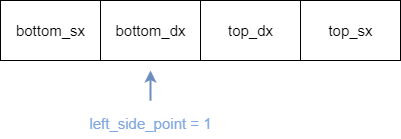
\includegraphics[width=0.5\linewidth]{immagini/array_vertici_puntatore.png}
            \caption{Variabile "puntatore" al vertice sul lato sinistro}
        \end{figure}
          Così facendo possiamo accedere facilmente anche ai punti sugli altri lati del box, ovvero:
          \begin{itemize}
              \item bottom\_side\_point = left\_side\_point + 1 \% 4.
              \item right\_side\_point = left\_side\_point + 2 \% 4.
              \item top\_side\_point = left\_side\_point + 3 \% 4.
          \end{itemize}
    \item Creiamo un nuovo array, in cui i vertici saranno disposti nello stesso ordine. Prendiamo il punto sul lato superiore come perno, quindi lasciamo le sue coordinate invariate. Il punto sul lato opposto, invece, manterrà stessa ascissa e avrà ordinata pari a \textit{box\_width}, ovvero la larghezza del box, poiché è la nuova altezza che vogliamo ottenere per rendere il box quadrato. Per quanto riguarda i due punti sui lati di sinistra e destra, andiamo a calcolare la seguente proporzione $$old\_y : box\_height = new\_y : box\_width.$$
          Il codice risultante sarà quindi:


          \begin{figure}[H]
            \centering
            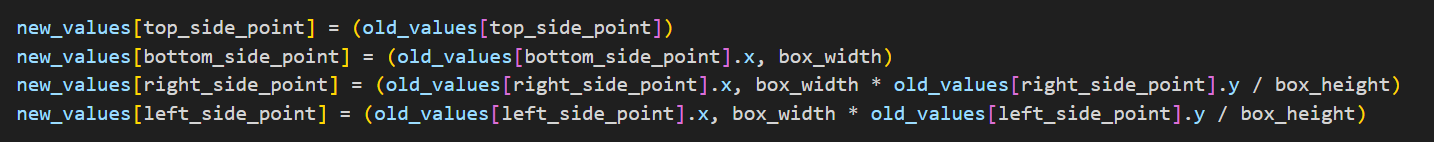
\includegraphics[width=\linewidth]{immagini/codice_interpolazione_vertici.png}
            \caption{Codice di calcolo dei vertici interpolati}
        \end{figure}


    \item A questo punto, possiamo calcolare l'angolo tra il vettore che parte da bottom\_dx e arriva a top\_dx, ovvero il vettore tra new\_values[1] e new\_values[2] e il vettore parallelo all'asse y rivolto verso il basso, ovvero (0, -1). Questo angolo sarà il valore assoluto del nostro yaw.
    \item Ciò che manca ora è il calcolo del segno dello yaw, che si può facilmente ricavare controllando l'orientamento del vettore sopra citato. Se l'ascissa della punta del vettore è maggiore dell'ascissa della base, allora lo yaw è positivo, altrimenti negativo.
\end{enumerate}
Di seguito una spiegazione geometrica dei calcoli eseguiti.
\begin{figure}[H]
    \centering
    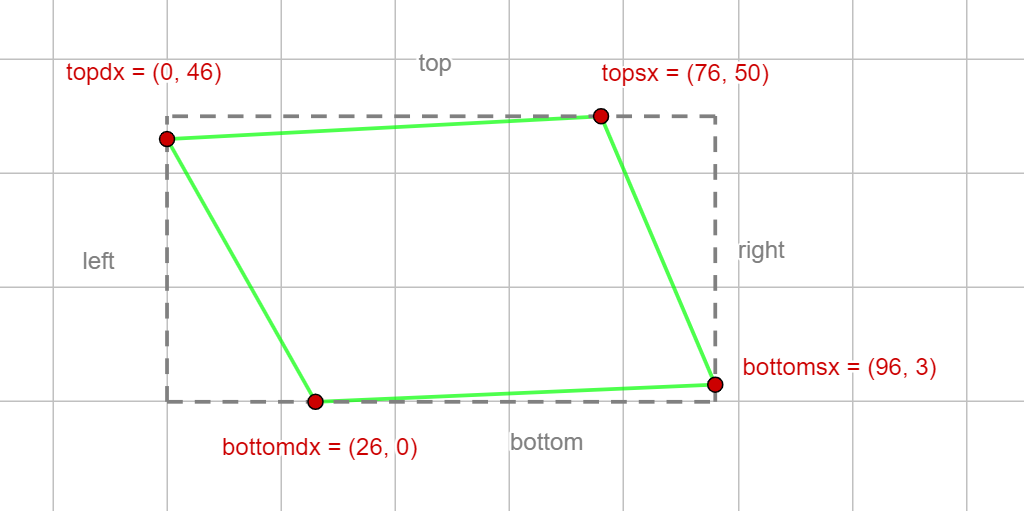
\includegraphics[width=0.4\linewidth]{immagini/tag_prima_dell_interpolazione.png}
    \caption{Tag originale all'interno del frame catturato}
\end{figure}
\begin{figure}[H]
    \centering
    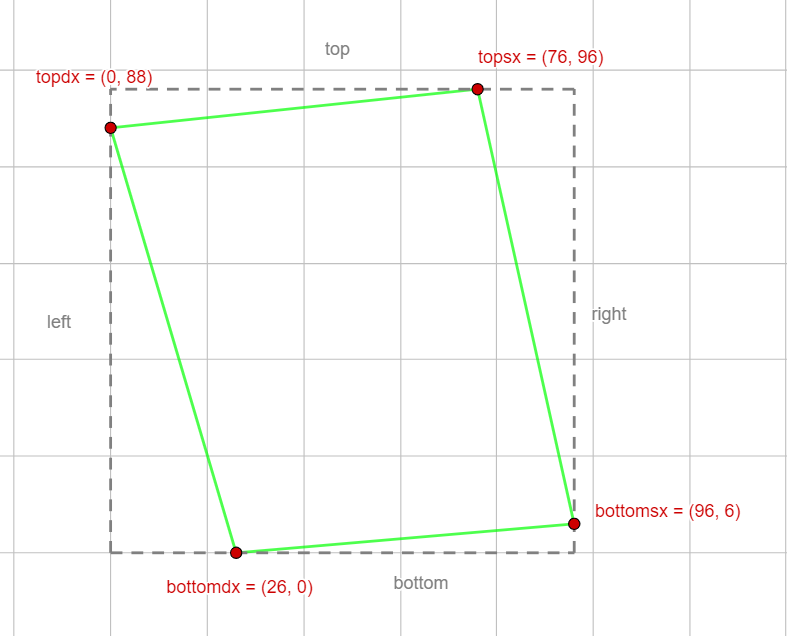
\includegraphics[width=0.4\linewidth]{immagini/tag_dopo_interpolazione.png}
    \caption{Tag interpolato}
\end{figure}
\begin{figure}[H]
    \centering
    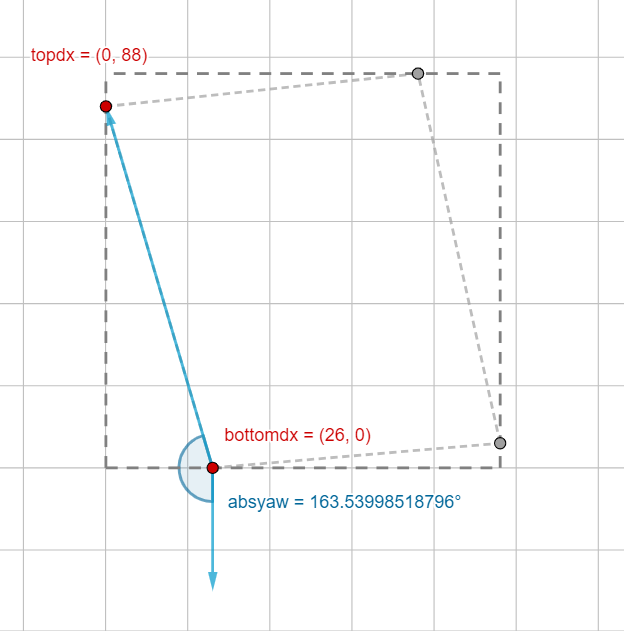
\includegraphics[width=0.4\linewidth]{immagini/calcolo_yaw.png}
    \caption{Calcolo dello yaw in valore assoluto}
\end{figure}

\subsubsection{Riduzione tempo di elaborazione tag sull'immagine}
L'ultimo problema riscontrato sull'odometria riguarda il tempo di elaborazione dei tag. Abbiamo notato infatti la presenza di un notevole ritardo tra la presenza di un tag di fronte al robot e la sua successiva elaborazione. Tale ritardo aveva ripercussioni sul movimento automatico, in quanto era come se il robot si muovesse basandosi su informazioni relative a mezzo secondo prima. Abbiamo eseguito quindi uno studio sui tempi di elaborazione, dividendo la porzione di codice dedicata all'elaborazione dei tag nei seguenti segmenti:
\begin{itemize}
    \item \textbf{Segmento 1}: comprende le operazioni di ritaglio della parte superiore dell'immagine e convoluzione con un filtro di sharpening.
    \item \textbf{Segmento 2}: comprende le operazioni di conversione in scala di grigi e thresholding.
    \item \textbf{Segmento 3:} comprende l'operazione di detection di AprilTags sull'immagine.
    \item \textbf{Segmento 4:} comprende l'operazione di salvataggio dell'immagine su disco solo se non sono stati rilevati tags.
    \item \textbf{Segmento 5:} comprende l'operazione di conversione dell'immagine da scala di grigi a colori, il disegno delle linee intorno al tag e il salvataggio dell'immagine su disco. I segmenti 5, 6 e 7 vengono eseguiti solo quando non viene eseguito il segmento 4.
    \item \textbf{Segmento 6:} comprende tutti i calcoli legati all'orientamento del tag, spiegati nel sottocapitolo precedente.
    \item \textbf{Segmento 7:} comprende la serializzazione dei dati ricavati dal tag in json.
\end{itemize}
Abbiamo quindi memorizzato i tempi per ogni segmento, ottenendo come risultato il seguente grafico
\begin{figure}[H]
    \centering
    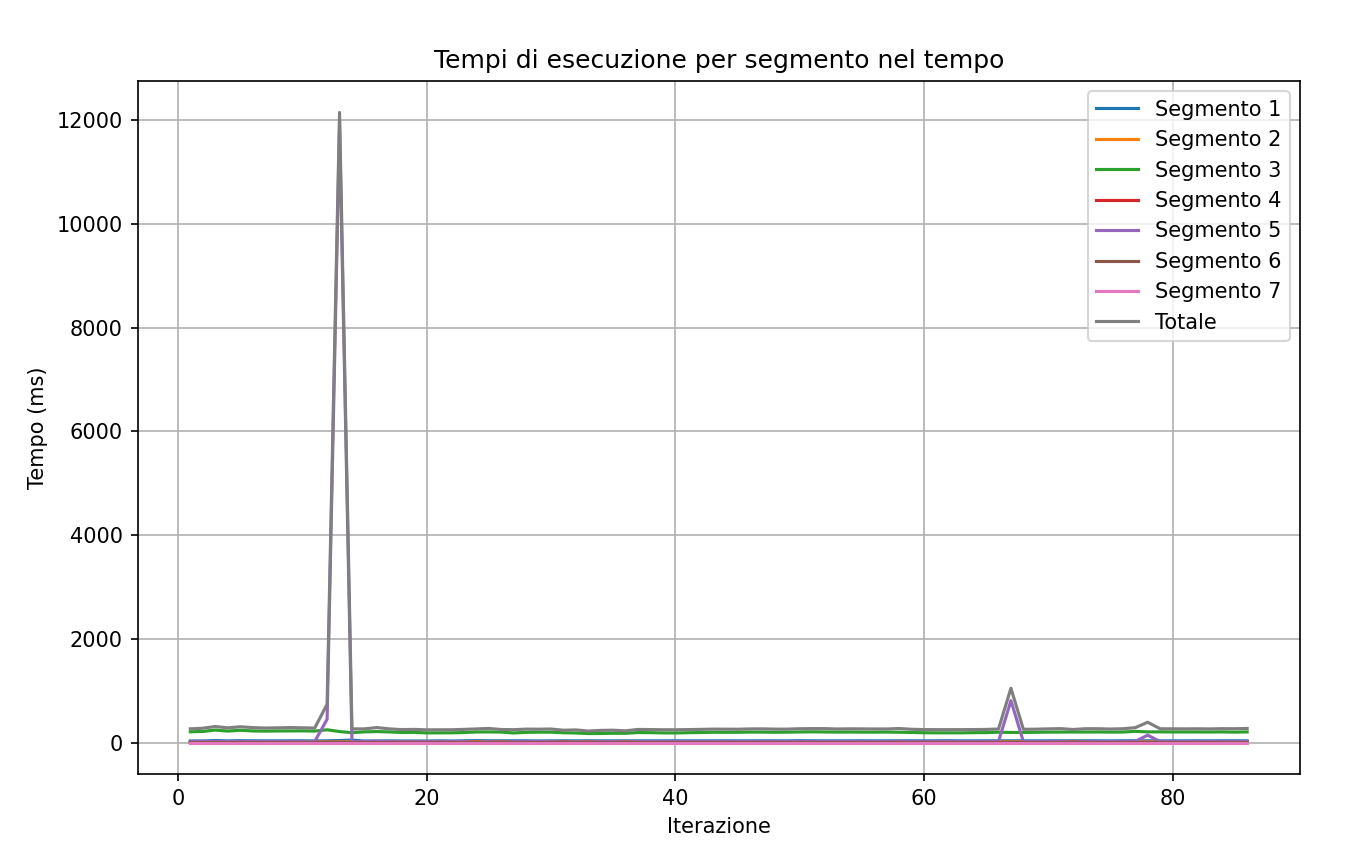
\includegraphics[width=0.7\linewidth]{immagini/grafico_tags_prima_delle_modifiche_intero.png}
    \caption{Grafico dei tempi di esecuzione}
\end{figure}
\begin{figure}[H]
    \centering
    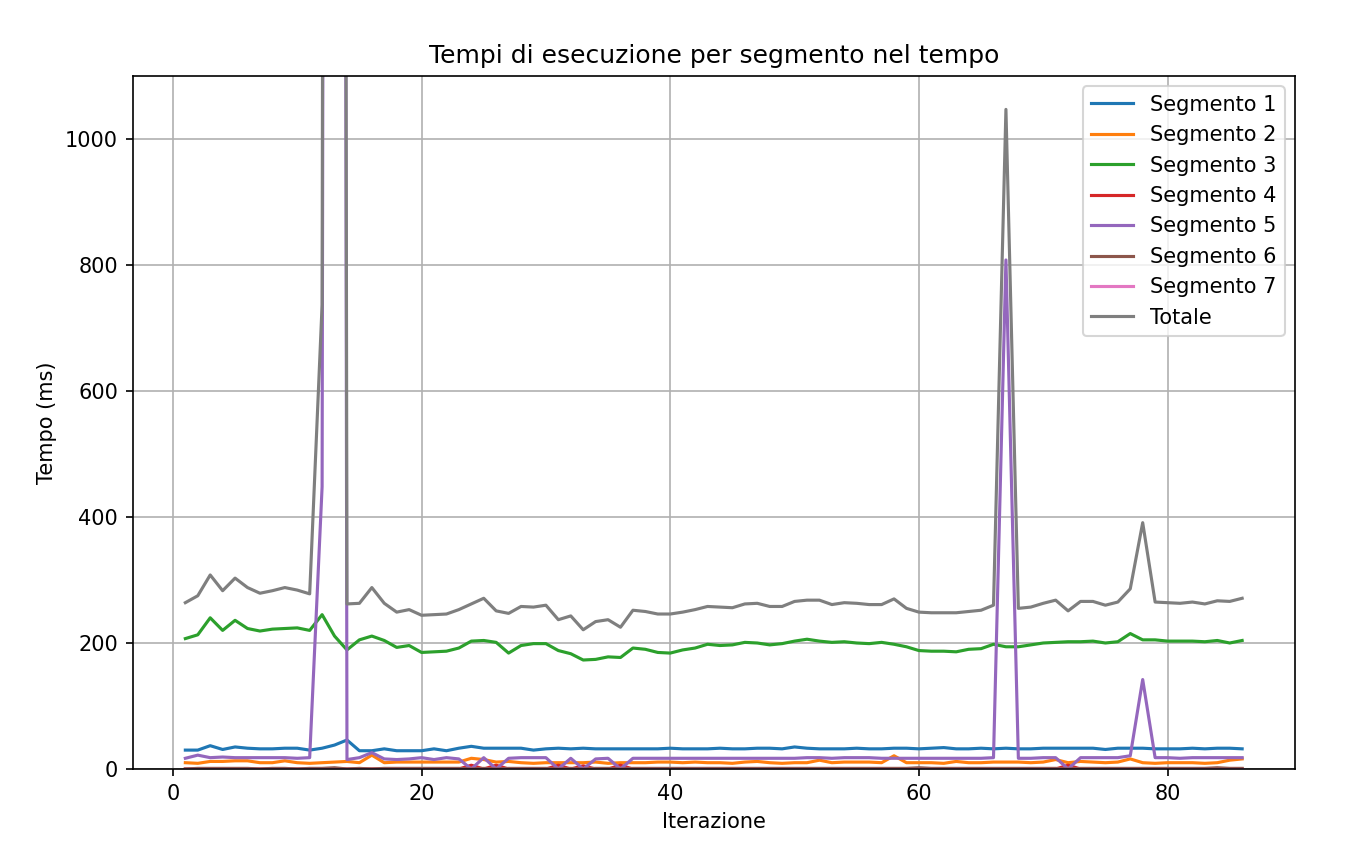
\includegraphics[width=0.7\linewidth]{immagini/grafico_tags_prima_delle_modifiche.png}
    \caption{Stesso grafico con la $y$ limitata a 1200 per mostrare meglio i tempi più bassi}
\end{figure}
e ricavato anche le seguenti statistiche
\begin{table}[H]
    \centering
    \begin{tabular}{lccc}
        \toprule
        Segmento & Minimo & Massimo & Media \\
        \midrule
        1        & 29     & 46      & 32    \\
        2        & 9      & 22      & 11    \\
        3        & 173    & 245     & 200   \\
        4        & 0      & 6       & 0     \\
        5        & 0      & 11892   & 170   \\
        6        & 0      & 2       & 1     \\
        7        & 0      & 0       & 0     \\
        \midrule
        Tot      & 221    & 12154   & 415   \\
        \bottomrule
    \end{tabular}
    \caption{Statistiche dei tempi di esecuzione}

\end{table}
Da questi dati possiamo notare diversi aspetti: il primo è che, per ogni frame catturato dalla telecamera, tra lo scatto e l'invio dei dati passano in media 4 decimi di secondo, ovvero una quantità di tempo enorme considerando la portata molto ridotta degli spostamenti che il robot deve compiere. Prendendo, ad esempio, il caso in cui il robot stia ruotando su se stesso, sappiamo che la velocità di rotazione è pari a 0.3 rad/s. Ciò significa che, con un ritardo di 0.4 s, il robot termina di processare le informazioni che ha ricevuto per un certo frame dopo aver ruotato di $0.3 * 0.4 \approx 7 \degree$. Dato che questo è solo l'overhead introdotto dall'elaborazione dei tag e che sicuramente ci saranno altre operazioni in tutto il processo che porta dalla lettura dei dati del tag all'attuazione dell'operazione calcolata, questo angolo sarà in realtà sicuramente maggiore.

Il secondo aspetto riguarda invece i picchi di massimo causati dal segmento 5, ovvero quello relativo al salvataggio dell'immagine su disco. È significativo notare come il massimo di questo segmento sia di ben 11.9 s, un lasso di tempo in cui il robot non ha possibilità di aggiornare la propria posizione e orientamento, muovendosi quindi alla cieca.

\subsubsection*{Risoluzione del problema}

Per risolvere questo problema abbiamo apportato due modifiche principali:
\begin{itemize}
    \item \textbf{Riduzione della dimensione dell'immagine} del 50\% per ogni lato, portando quindi ad una riduzione del 75\% sull'area. Ciò avrebbe dovuto portare infatti ad una riduzione del tempo di esecuzione principalmente della detection e dello sharpening, essendo due operazioni basate su convoluzione e altre operazioni tra matrici.
    \item \textbf{Spostamento dell'operazione di salvataggio dell'immagine} su thread separato, senza curarsi del risultato finale. Dato che, infatti, il salvataggio dell'immagine serve solo per mostrare a noi ciò che il robot vede, e che non ha uno scopo rispetto alla corretta esecuzione, non è un problema se qualche frame viene perso  sovrascritto.
\end{itemize}
Dopo queste modifiche, ecco i dati relativi ai segmenti aggiornati:

\begin{figure}[H]
    \centering
    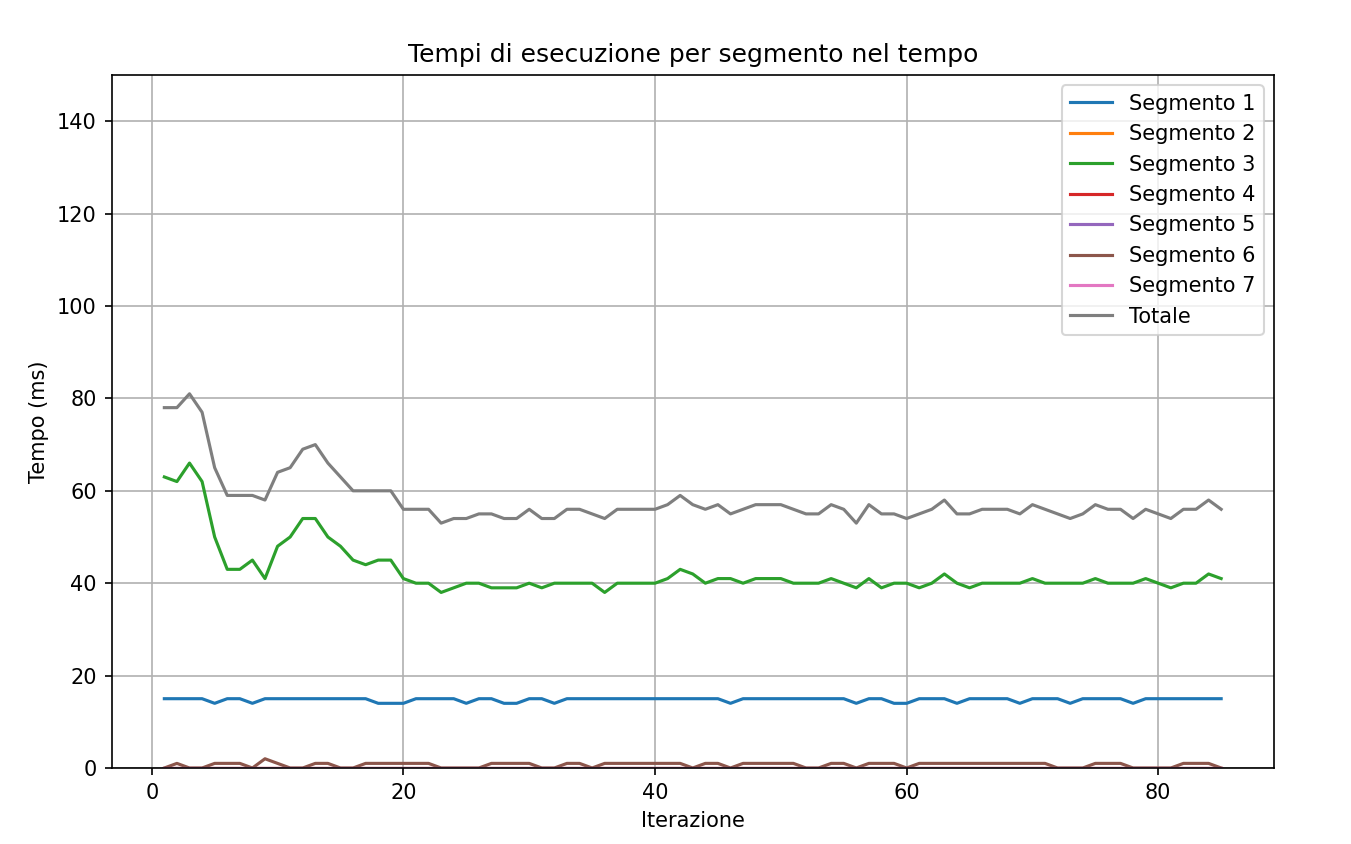
\includegraphics[width=0.7\linewidth]{immagini/grafico_tags_dopo_le_modifiche.png}
    \caption{Grafico dei tempi di esecuzione dopo i miglioramenti}
\end{figure}

\begin{table}[H]
    \centering
    \begin{tabular}{lccc}
        \toprule
        Segmento & Minimo & Massimo & Media \\
        \midrule
        1        & 14     & 15      & 15    \\
        2        & 0      & 0       & 0     \\
        3        & 38     & 66      & 42    \\
        4        & 0      & 0       & 0     \\
        5        & 0      & 0       & 0     \\
        6        & 0      & 2       & 1     \\
        7        & 0      & 0       & 0     \\
        \midrule
        Tot      & 53     & 81      & 58    \\
        \bottomrule
    \end{tabular}
    \caption{Statistiche dopo i miglioramenti}
\end{table}

Notiamo un drastico calo dei tempi di esecuzione e la completa eliminazione dei picchi di massimo, ottenendo quindi un overhead accettabile ai fini dell'esecuzione. È interessante notare inoltre come il tempo di esecuzione del segmento 3 (detection degli AprilTags) aumenti linearmente con l'area dell'immagine: infatti, dopo una riduzione del 75\% dell'area dell'immagine, anche il tempo di esecuzione medio della detection è sceso di circa il 75\%.

\subsection{Rilevamento ostacoli}

\subsubsection{Camera di profondità}
Per il rilevamento degli ostacoli, la prima idea è stata quella di utilizzare la camera di profondità, ma a causa di un problema firmware delle Astra più vecchie del 2017, avevamo dei valori non realistici e quindi errori nel rilevamento.

\subsubsection{Sensori ad infrarossi}
Successivamente abbiamo sostituito la camera con tre sensori ad infrarossi collegati direttamente con il Raspberry Pi. Uno script Python si occupava di leggerne i valori
ed inviarli al modulo delle percezioni. Purtroppo anche questo approccio è stato scartato per via della distanza massima molto corta e delle continue interferenze
dovute alla sensibilità troppo alta dei sensori.

\subsubsection{Sensori ad ultrasuoni fissi}
Siamo passati quindi all'utilizzo di cinque sensori ad ultrasuoni, uno per ogni direzione di movimento, fissati sul contorno frontale del robot. Il problema di questa soluzione era che i sensori coprivano un angolo quasi nullo, coprendo un'area simile ad un cilindro. Questo portava ad avere dei vuoti tra i sensori e quindi dei punti ciechi per il robot.

\subsubsection{Sonar ad ultrasuoni}
La soluzione finale è stata quella di implementare tre sonar ruotanti, grazie all'applicazione dei sensori a ultrasuoni su tre servomotori. Grazie a tale rotazione, l'angolo coperto dai sensori va a raggiungere i 70° per sensore, per un totale di 210° di copertura. Un ultimo problema di questa soluzione è stato ancora legato al cilindro dei sensori, ma in "verso opposto". Il cilindro infatti, seppur molto stretto, andava comunque a coprire una superficie rettangolare di larghezza simile a quella della base del sensore. Ciò portava ad una distorsione dei dati letti, in quanto, ad esempio, il dato rilevato quando l'angolo era di 55°, non era quello corrispondente all'esatto punto che si trovava a 55°, ma anche ai gradi in un certo vicinato. La soluzione finale è stata quindi quella di disporre i sensori in verticale sui servomotori, in modo da diminuire l'estensione orizzontale del sensore e al tempo stesso ottenere un aumento della copertura verticale degli stessi.

\subsection{Algoritmo di obstacle avoidance}
Una volta rilevati gli ostacoli, al controller viene comunicato quali spazi sono liberi tra le direzioni di movimenti possibili. Il calcolo di tali spazi liberi dipende chiaramente dalla distanza degli ostacoli. Tale calcolo è stato evoluto durante lo sviluppo del progetto, fino ad arrivare alla soluzione finale.



\subsubsection{Calcolo degli spazi liberi}
Il modulo perception riceve dei valori numerici dai sensori: per ogni direzione di movimento, viene restituito il valore pari alla distanza tra il sensore e l'ostacolo più vicino rilevato. Dati questi valori, il compito del modulo perception è quello di elaborare tali dati e settare un flag di spazio libero per ogni direzione. Il settaggio di questi flag dipende da quanto il sensore è lontano.

\subsubsection*{Prima soluzione}
In un primo momento, questo calcolo veniva fatto basandosi su una singola soglia: se il sensore in direzione X restituiva un valore minore rispetto alla soglia, allora lo spazio relativo alla direzione X veniva impostato come non libero. Questa soluzione era poco affidabile, poiché se un ostacolo si è più vicino potrebbe bloccare anche altre direzioni a causa della grandezza del robot.

\subsubsection*{Soluzione finale}
La soluzione finale prevede l'utilizzo di tre soglie: long\_distance, medium\_distance e short\_distance. Queste soglie vengono utilizzate nel seguente modo:
\begin{itemize}
    \item Se il valore del sensore in direzione X è compreso tra long\_distance e medium\_distance, allora viene impostato a false solo lo spazio in direzione X.
    \item Se il valore del sensore X è compreso tra medium\_distance e short\_distance, allora viene impostato a false lo spazio in direzione X ed i due adiacenti.
    \item Se il valore del sensore X è minore di short\_distance, allora imposto a false tutte le direzioni frontali e in più, se last\_command è diverso da FRONT, anche la direzione laterale più vicina (es: se last\_command è FRONTRIGHT, blocco RIGHT.)
\end{itemize}
Questa soluzione rende più flessibile la scelta della direzione finale e prende in considerazione anche la grandezza del robot.

\begin{figure}[H]
    \centering
    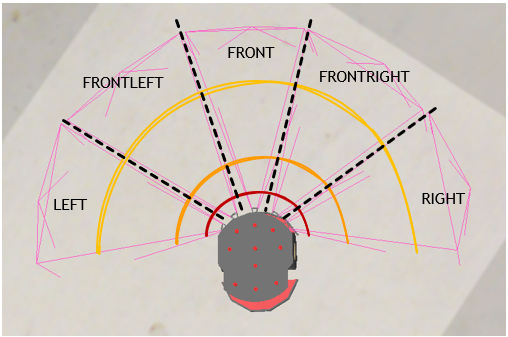
\includegraphics[width=0.6\linewidth]{immagini/soglie_obstacle_avoidance.png}
    \caption{Rappresentazione grafica delle soglie}
    
\end{figure}

\subsubsection{Scelta della direzione da percorrere}
A seconda della modalità di movimento che si sta utilizzando, il calcolo del comando da eseguire avviene in modo diverso. Una volta scelto tale comando, che da ora chiameremo \textit{last\_command}, esso passerà per l'algoritmo di obstacle avoidance. Supposto che gli spazi liberi sono già stati calcolati, l'algoritmo agisce nel seguente modo:
\begin{enumerate}
    \item Se la direzione last\_command è libera, allora prosegue in quella direzione.
    \item Se la direzione last\_command è occupata, allora vengono controllate le direzioni adiacenti, in un ordine che dipende da che direzione è contenuta in last\_command, ovvero:


          \begin{table}[H]
              \centering
              \begin{tabular}{|c|c|c|}
                  \hline
                  \textbf{Last Command}                & \textbf{Modalità}   & \textbf{Azione}                                \\
                  \hline
                  \texttt{FRONT}                       & -                   & \texttt{(FRONTLEFT, FRONTRIGHT, LEFT, RIGHT)}  \\
                  \hline
                  \multirow{2}{*}{\texttt{FRONTLEFT}}  & \texttt{Manuale}    & \texttt{(LEFT, FRONT, FRONTRIGHT, RIGHT)}      \\

                  \cline{2-3}
                                                       & \texttt{Automatica} & \texttt{(FRONT, FRONTRIGHT, RIGHT, LEFT)}      \\
                  \hline
                  \multirow{2}{*}{\texttt{FRONTRIGHT}} & \texttt{Manuale}    & \texttt{(RIGHT, FRONT, FRONTLEFT, LEFT)}       \\
                  \cline{2-3}
                                                       & \texttt{Automatica} & \texttt{(FRONT, FRONTLEFT, LEFT, RIGHT)}       \\
                  \hline

                  \texttt{LEFT}                        & -                   & \texttt{(FRONTLEFT, FRONT, FRONTRIGHT, RIGHT)} \\
                  \hline
                  \texttt{RIGHT}                       & -                   & \texttt{(FRONTRIGHT, FRONT, FRONTLEFT, LEFT)}  \\
                  \hline
              \end{tabular}
              \caption{Valutazione delle direzioni adiacenti}
          \end{table}
\end{enumerate}

\pagebreak
\section{Obiettivi raggiunti}

Siamo riusciti ad implementare quasi tutte le funzionalità che ci eravamo imposti. Purtroppo nella parte fisica l'obstacle avoidance
in combinazione con la modalità automatica soffre ancora di numerosi problemi ed è pressochè inutilizzabile.
I numerosi imprevisti avvenuti soprattuto verso la fine ci hanno impedito di impementare correttamente questo requisito.
Nonostante ciò siamo molto fieri dei risultati ottenuti visto soprattutto la nostra limitata esperienza in tale ambito.

\section{Codice sorgente}

Repository git con il nostro codice: \href{https://github.com/luca-tracanna/gesture\_driven\_robot}{https://github.com/luca-tracanna/gesture\_driven\_robot}

\pagebreak
\printbibliography

\end{document}